%% (Master) Thesis template
% Template version used: v1.4
%
% Largely adapted from Adrian Nievergelt's template for the ADPS
% (lecture notes) project.

\PassOptionsToPackage{dvipsnames}{xcolor}

%% We use the memoir class because it offers many easy to use features.
\documentclass[11pt,a4paper,titlepage]{memoir}

%% Packages
%% ========

%% LaTeX Font encoding -- DO NOT CHANGE
\usepackage[OT1]{fontenc}

%% Babel provides support for languages.  'english' uses British
%% English hyphenation and text snippets like "Figure" and
%% "Theorem". Use the option 'ngerman' if your document is in German.
%% Use 'american' for American English.  Note that if you change this,
%% the next LaTeX run may show spurious errors.  Simply run it again.
%% If they persist, remove the .aux file and try again.
\usepackage[american]{babel}

%% Input encoding 'utf8'. In some cases you might need 'utf8x' for
%% extra symbols. Not all editors, especially on Windows, are UTF-8
%% capable, so you may want to use 'latin1' instead.
\usepackage[utf8]{inputenc}

%% This changes default fonts for both text and math mode to use Herman Zapfs
%% excellent Palatino font.  Do not change this.
\usepackage[sc]{mathpazo}

%% The AMS-LaTeX extensions for mathematical typesetting.  Do not
%% remove.
\usepackage{amsmath,amssymb,amsfonts,mathrsfs}

%% NTheorem is a reimplementation of the AMS Theorem package. This
%% will allow us to typeset theorems like examples, proofs and
%% similar.  Do not remove.
%% NOTE: Must be loaded AFTER amsmath, or the \qed placement will
%% break
\usepackage[amsmath,thmmarks]{ntheorem}

%% LaTeX' own graphics handling
\usepackage{graphicx}
\graphicspath{{figures/}} %tell package where to find graphics


%% We unfortunately need this for the Rules chapter.  Remove it
%% afterwards; or at least NEVER use its underlining features.
\usepackage{soul}

%% This allows you to add .pdf files. It is used to add the
%% declaration of originality.
\usepackage{pdfpages}

\usepackage{xspace}

\usepackage{capt-of}

\usepackage{float}

\usepackage[section]{placeins}

\usepackage{subfig}

\usepackage[square, comma, sort&compress, numbers]{natbib}
%% Some more packages that you may want to use.  Have a look at the
%% file, and consult the package docs for each.
%% See the TeXed file for more explanations

%% [OPT] Multi-rowed cells in tabulars
%\usepackage{multirow}

%% [REC] Intelligent cross reference package. This allows for nice
%% combined references that include the reference and a hint to where
%% to look for it.
\usepackage{varioref}

%% [OPT] Easily changeable quotes with \enquote{Text}
%\usepackage[german=swiss]{csquotes}

%% [REC] Format dates and time depending on locale
\usepackage{datetime}

%% [OPT] Provides a \cancel{} command to stroke through mathematics.
%\usepackage{cancel}

%% [NEED] This allows for additional typesetting tools in mathmode.
%% See its excellent documentation.
\usepackage{mathtools}

%% [ADV] Conditional commands
%\usepackage{ifthen}

%% [OPT] Manual large braces or other delimiters.
%\usepackage{bigdelim, bigstrut}

%% [REC] Alternate vector arrows. Use the command \vv{} to get scaled
%% vector arrows.
\usepackage[h]{esvect}

%% [NEED] Some extensions to tabulars and array environments.
\usepackage{array}

%% [OPT] Postscript support via pstricks graphics package. Very
%% diverse applications.
%\usepackage{pstricks,pst-all}

%% [?] This seems to allow us to define some additional counters.
%\usepackage{etex}

%% [ADV] XY-Pic to typeset some matrix-style graphics
%\usepackage[all]{xy}

%% [OPT] This is needed to generate an index at the end of the
%% document.
%\usepackage{makeidx}

%% [OPT] Fancy package for source code listings.  The template text
%% needs it for some LaTeX snippets; remove/adapt the \lstset when you
%% remove the template content.
%% Settings for code listings
\usepackage{listings}
\usepackage{listings-golang}
\lstset{ % add your own preferences
	frame=single,
	basicstyle=\footnotesize,
	keywordstyle=\color{violet},
	commentstyle=\color{OliveGreen},
	numbers=left,
	numbersep=5pt,
	showstringspaces=false, 
	stringstyle=\color{magenta},
	tabsize=4,
	language=golang
}

\lstdefinelanguage{yaml}
{
 morekeywords=[1]{mysql_db,mysql_pass,apt,name,password,host,login_password,mysql_db,mysql_user,with_items,jobs,build,docker,image,environment,MYSQL_ROOT_PASSWORD,MYSQL_DATABASE,steps,run,command,working_directory,version},
	sensitive=true,
	morestring=[b]",
%	morecomment=[l]:,
}

\lstset{ % add your own preferences
	frame=single,
	basicstyle=\footnotesize,
	keywordstyle=\color{blue},
	commentstyle=\color{OliveGreen},
	moredelim = [l][\functionColonHighlight]{:}{ljl}
	numbers=left,
	numbersep=5pt,
	showstringspaces=false, 
	stringstyle=\color{magenta},
	tabsize=4,
	language=yaml
}

\newcommand{\functionColonHighlight}[1]{\bfseries\textcolor{blue}{:} \textcolor{magenta}{\mdseries #1}(}



%% [REC] Fancy character protrusion.  Must be loaded after all fonts.
\usepackage[activate]{pdfcprot}

%% [REC] Nicer tables.  Read the excellent documentation.
\usepackage{booktabs}


%% Our layout configuration.  DO NOT CHANGE.
%% Memoir layout setup

%% NOTE: You are strongly advised not to change any of them unless you
%% know what you are doing.  These settings strongly interact in the
%% final look of the document.

% Dependencies
\usepackage{ETHlogo}

% Turn extra space before chapter headings off.
\setlength{\beforechapskip}{0pt}

\nonzeroparskip
\parindent=0pt
\defaultlists

% Chapter style redefinition
\makeatletter

\if@twoside
  \pagestyle{Ruled}
  \copypagestyle{chapter}{Ruled}
\else
  \pagestyle{ruled}
  \copypagestyle{chapter}{ruled}
\fi
\makeoddhead{chapter}{}{}{}
\makeevenhead{chapter}{}{}{}
\makeheadrule{chapter}{\textwidth}{0pt}
\copypagestyle{abstract}{empty}

\makechapterstyle{bianchimod}{%
  \chapterstyle{default}
  \renewcommand*{\chapnamefont}{\normalfont\Large\sffamily}
  \renewcommand*{\chapnumfont}{\normalfont\Large\sffamily}
  \renewcommand*{\printchaptername}{%
    \chapnamefont\centering\@chapapp}
  \renewcommand*{\printchapternum}{\chapnumfont {\thechapter}}
  \renewcommand*{\chaptitlefont}{\normalfont\huge\sffamily}
  \renewcommand*{\printchaptertitle}[1]{%
    \hrule\vskip\onelineskip \centering \chaptitlefont\textbf{\vphantom{gyM}##1}\par}
  \renewcommand*{\afterchaptertitle}{\vskip\onelineskip \hrule\vskip
    \afterchapskip}
  \renewcommand*{\printchapternonum}{%
    \vphantom{\chapnumfont {9}}\afterchapternum}}

% Use the newly defined style
\chapterstyle{bianchimod}

\setsecheadstyle{\Large\bfseries\sffamily}
\setsubsecheadstyle{\large\bfseries\sffamily}
\setsubsubsecheadstyle{\bfseries\sffamily}
\setparaheadstyle{\normalsize\bfseries\sffamily}
\setsubparaheadstyle{\normalsize\itshape\sffamily}
\setsubparaindent{0pt}

% Set captions to a more separated style for clearness
\captionnamefont{\sffamily\bfseries\footnotesize}
\captiontitlefont{\sffamily\footnotesize}
\setlength{\intextsep}{16pt}
\setlength{\belowcaptionskip}{1pt}

% Set section and TOC numbering depth to subsection
\setsecnumdepth{subsection}
\settocdepth{subsection}

%% Titlepage adjustments
\pretitle{\vspace{0pt plus 0.7fill}\begin{center}\HUGE\sffamily\bfseries}
\posttitle{\end{center}\par}
\preauthor{\par\begin{center}\let\and\\\Large\sffamily}
\postauthor{\end{center}}
\predate{\par\begin{center}\Large\sffamily}
\postdate{\end{center}}

\def\@advisors{}
\newcommand{\advisors}[1]{\def\@advisors{#1}}
\def\@department{}
\newcommand{\department}[1]{\def\@department{#1}}
\def\@thesistype{}
\newcommand{\thesistype}[1]{\def\@thesistype{#1}}

\renewcommand{\maketitlehooka}{\noindent\ETHlogo[2in]}

\renewcommand{\maketitlehookb}{\vspace{1in}%
  \par\begin{center}\Large\sffamily\@thesistype\end{center}}

\renewcommand{\maketitlehookd}{%
  \vfill\par
  \begin{flushright}
    \sffamily
    \@advisors\par
    \@department, ETH Z\"urich
  \end{flushright}
}

\checkandfixthelayout

\setlength{\droptitle}{-48pt}

\makeatother

% This defines how theorems should look. Best leave as is.
\theoremstyle{plain}
\setlength\theorempostskipamount{0pt}

%%% Local Variables:
%%% mode: latex
%%% TeX-master: "thesis"
%%% End:


%% Theorem environments.  You will have to adapt this for a German
%% thesis.
%% Theorem-like environments

%% This can be changed according to language. You can comment out the ones you
%% don't need.

\numberwithin{equation}{chapter}

%% German theorems
%\newtheorem{satz}{Satz}[chapter]
%\newtheorem{beispiel}[satz]{Beispiel}
%\newtheorem{bemerkung}[satz]{Bemerkung}
%\newtheorem{korrolar}[satz]{Korrolar}
%\newtheorem{definition}[satz]{Definition}
%\newtheorem{lemma}[satz]{Lemma}
%\newtheorem{proposition}[satz]{Proposition}

%% English variants
\newtheorem{theorem}{Theorem}[chapter]
\newtheorem{example}[theorem]{Example}
\newtheorem{remark}[theorem]{Remark}
\newtheorem{corollary}[theorem]{Corollary}
\newtheorem{definition}[theorem]{Definition}
\newtheorem{lemma}[theorem]{Lemma}
\newtheorem{proposition}[theorem]{Proposition}

%% Proof environment with a small square as a "qed" symbol
\theoremstyle{nonumberplain}
\theorembodyfont{\normalfont}
\theoremsymbol{\ensuremath{\square}}
\newtheorem{proof}{Proof}
%\newtheorem{beweis}{Beweis}


%% Helpful macros.
%% Custom commands
%% ===============

%% Special characters for number sets, e.g. real or complex numbers.
\newcommand{\C}{\mathbb{C}}
\newcommand{\K}{\mathbb{K}}
\newcommand{\N}{\mathbb{N}}
\newcommand{\Q}{\mathbb{Q}}
\newcommand{\R}{\mathbb{R}}
\newcommand{\Z}{\mathbb{Z}}
\newcommand{\X}{\mathbb{X}}

%% Fixed/scaling delimiter examples (see mathtools documentation)
\DeclarePairedDelimiter\abs{\lvert}{\rvert}
\DeclarePairedDelimiter\norm{\lVert}{\rVert}

%% Use the alternative epsilon per default and define the old one as \oldepsilon
\let\oldepsilon\epsilon
\renewcommand{\epsilon}{\ensuremath\varepsilon}

%% Also set the alternate phi as default.
\let\oldphi\phi
\renewcommand{\phi}{\ensuremath{\varphi}}

\newcommand{\lee}{\textit{SCIONLab Experimentation Environment}\xspace}
\newcommand{\lcs}{\textit{SCIONLab Coordination Service}\xspace}
\newcommand{\lmi}{\textit{Local Management Service}\xspace}
\newcommand{\cords}{\textit{Coordination Service}\xspace}
\newcommand{\fnurl}[2]{\href{#2}{#1}\footnote{\url{#2}}\xspace}
\newcommand{\fnote}[2]{#1\footnote{#2}}\xspace
\newcommand{\fnoteurl}[3]{\href{#2}{#1}\footnote{{#3:} \url{#2}}\xspace}
\newcommand{\code}[1]{\colorbox{lightgray}{\textit{"#1"}}\xspace}
\newif\ifcomment
\newcommand{\cmnt}[1]{\ifcomment {\color{orange}{#1}} \fi}


\newcommand{\customtoday}{\ifcase \month \or January \or February \or March \or %
	April \or May \or June \or July \or August \or September \or October \or November \or %
	December \fi \number \day, \number \year} 


%% Make document internal hyperlinks wherever possible. (TOC, references)
%% This MUST be loaded after varioref, which is loaded in 'extrapackages'
%% above.  We just load it last to be safe.
\usepackage[linkcolor=black,colorlinks=true,citecolor=black,filecolor=black]{hyperref}

%% Document information
%% ====================

%%render comments
\commenttrue

\title{\LARGE{Mondrian: A Comprehensive Inter-Domain Network Zoning Architecture}}
\author{Claude Hähni}
\thesistype{Master Thesis}
\advisors{Advisors: Prof.\ Dr.\ Adrian Perrig, Dr.\ Jonghoon Kwon, Patrick Bamert}
\department{Department of Computer Science}
\date{\customtoday} % replace with fixed date once submission is done

\begin{document}

\frontmatter

%% Title page is autogenerated from document information above.  DO
%% NOT CHANGE.
\begin{titlingpage}
	\calccentering{\unitlength}
	\begin{adjustwidth*}{\unitlength-24pt}{-\unitlength-24pt}
		\maketitle
	\end{adjustwidth*}
\end{titlingpage}

%% The abstract of your thesis.  Edit the file as needed.
\begin{abstract}
        Large Reasoning Models (LRMs) represent a breakthrough in AI problem-solving capabilities, but their effectiveness in interactive environments may be limited. This thesis introduces and analyzes \textbf{overthinking} in LRMs—a phenomenon where models favor extended internal reasoning chains over environmental interaction. Through experiments on software engineering tasks using SWE Bench Verified, we observe three recurring patterns: \textit{Analysis Paralysis, Rogue Actions, and Premature Disengagement}. We propose a framework to study these behaviors, which correlates with human expert assessments, and analyze \textbf{3,908 trajectories}. We observe that higher overthinking scores correlate with decreased performance, with reasoning models exhibiting stronger tendencies toward overthinking compared to non-reasoning models. Our analysis reveals that simple solutions—such as selecting solutions with lower overthinking scores—can \textbf{improve model performance by 25\% while decreasing computational costs by 43\%}. Based on these findings, we suggest promising directions for mitigating overthinking through native function-calling capabilities and selective reinforcement learning, potentially offering a path to better balance reasoning and environmental interaction. To facilitate further research in this direction, we open-source our evaluation framework and dataset.
\end{abstract}

\addcontentsline{toc}{section}{Abstract}
\newpage

%% The acknowledgements
\renewcommand{\abstractname}{Acknowledgments}
\begin{abstract}
	First and foremost, I would like to thank Prof. Dr. Adrian Perrig for providing me the opportunity of working
	on this fascinating project. His continued support is very appreciated.

	I would like to express my sincere gratitude to Dr. Jonghoon Kwon and Patrick Bamert for the
	many discussions and valuable insights. Without their help, this thesis would not have been possible.

	Lastly, my special thank goes to my family and friends for their unconditional support throughout
	my studies.
\end{abstract}

\addcontentsline{toc}{section}{Acknowledgments}
\newpage

%% Citing the paper
\renewcommand{\abstractname}{Preface}
\begin{abstract}
	The work done in this thesis has additionally been submitted as research
	paper~\cite{kwon2020Mondrian}. At the time of writing, the manuscript has
	been submitted and is undergoing review.
	This thesis aims to expand on the paper, giving deeper insights into the different aspects of \name.
\end{abstract}

\addcontentsline{toc}{section}{Preface}

%% TOC with the proper setup, do not change.
\cleartorecto
\tableofcontents
\mainmatter

%% Your real content!
\chapter{Introduction}
\label{intro}

Large Reasoning Models (LRMs) represent a breakthrough in AI problem-solving capabilities, yet their effectiveness in interactive environments remains poorly understood. This thesis introduces and analyzes the phenomenon of \textbf{overthinking} in LRMs - a tendency where models prioritize elaborate internal simulations of potential actions over gathering actual environmental feedback. Through extensive experiments on software engineering tasks using SWE Bench Verified, we develop a systematic framework to quantify overthinking behavior on a 0-10 scale, measuring how models balance internal reasoning chains against environmental interaction.

\begin{figure}[t]
    \centering
    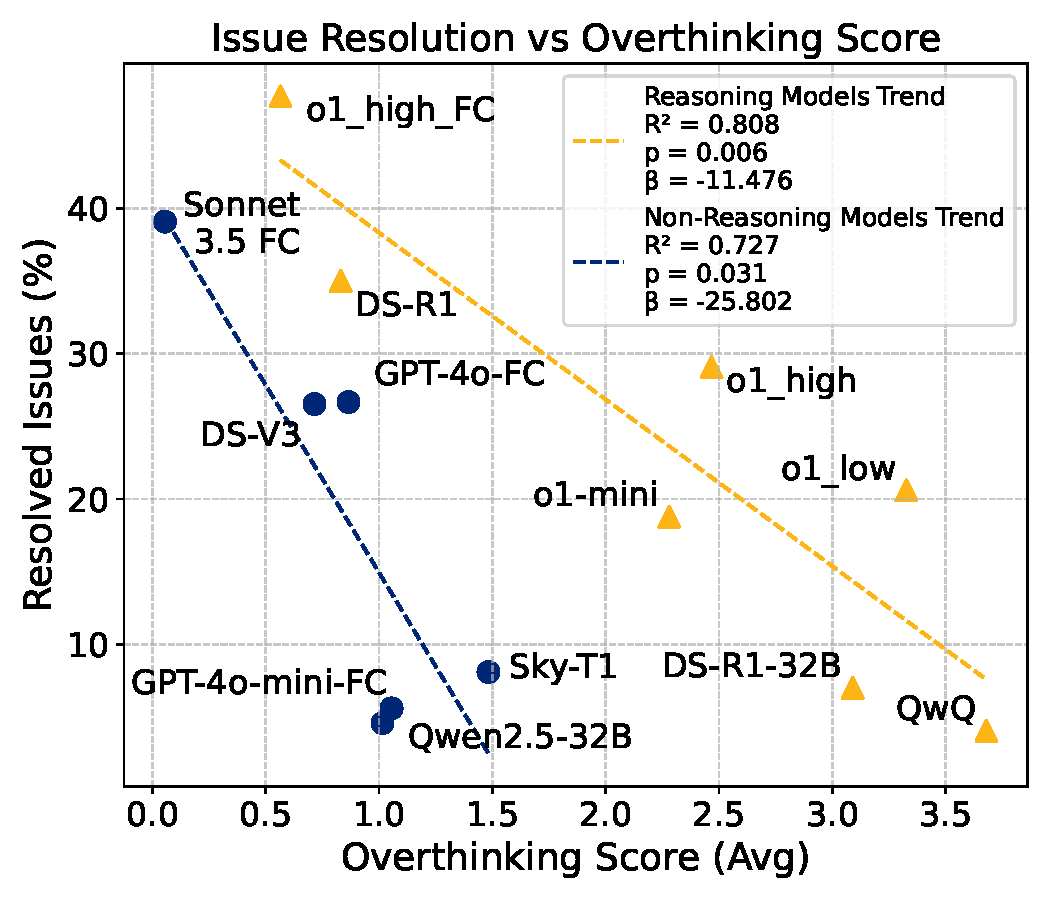
\includegraphics[width=1\linewidth]{model_analysis_combined.pdf}
    \caption{Higher overthinking scores (tendency to favor internal reasoning over environmental feedback) correlate with lower issue resolution rates across all models. Reasoning models exhibit consistently higher overthinking tendencies, suggesting that excessive reliance on internal simulation impairs task performance. Model nomenclature: "FC" indicates native function calling capability, "DS" represents DeepSeek models, and suffixes o1\_high and o1\_low denote models with reasoning effort set to high and low respectively.}
    \label{fig:figure1}
\end{figure}

\begin{figure}[t]
    \centering
    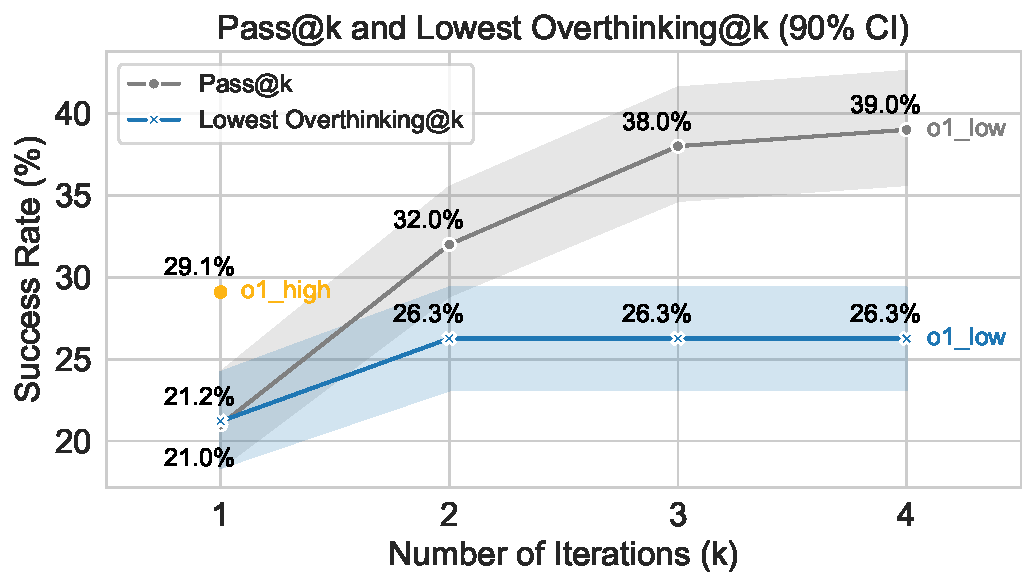
\includegraphics[width=1\linewidth]{pass_at_k_plot.pdf}
    \caption{Pass@k performance for SWE Bench Verified when selecting responses based on overthinking scores. By choosing solutions with minimal overthinking from multiple runs of o1 with low reasoning effort, we achieve performance comparable to high reasoning effort configurations at substantially lower computational cost. The flattening curve suggests diminishing returns from additional iterations, with detailed performance metrics provided in \cref{tab:o1_model_comparison}. The confidence intervals (CI) showcased were computed using Wilson score.}
    \label{fig:figure2}
\end{figure}

Analysis of \textbf{3,908 trajectories} reveals that overthinking significantly impairs model performance, with strong negative correlations between overthinking scores and issue resolution capabilities (R² = 0.808, p = 0.006 for reasoning models). Notably, LRMs exhibit higher overthinking scores (2.320 ± 1.120) compared to non-reasoning models (0.865 ± 0.432, p = 0.019). Based on our findings, we propose that integrating native function-calling capabilities during training may help models better balance reasoning and action.

\section{The Rise of Large Reasoning Models}
LRMs, defined as LLMs leveraging reinforcement learning techniques for train-time scaling, represent a breakthrough in AI reasoning capabilities. These models are fundamentally built on the principle that allocating more computational resources at test-time enables deeper reasoning. This approach has proven remarkably effective: by dedicating significant compute to deliberate reasoning steps, these models achieve unprecedented performance through extended chain-of-thought reasoning, systematic exploration of solution strategies, and rigorous self-verification. However, this extended focus on internal reasoning depth raises important questions about how these models balance internal deliberation with action in interactive environments.

\section{The Challenge of Agentic Environments}
While traditional AI defined agents broadly as entities that perceive and act upon their environment, the LLM era has evolved toward viewing agency as a spectrum of capabilities. Systems are considered more agentic based on three key factors:
\begin{itemize}
    \item Their ability to handle complex environments and pursue goals autonomously
    \item Their capacity to act with minimal supervision through natural language interfaces
    \item Their use of advanced design patterns such as tool utilization and dynamic planning
\end{itemize}

These principles have been extensively applied to software engineering tasks, particularly in solving real-world GitHub issues, where numerous research efforts have explored different agent architectures with varying degrees of success. While these efforts have advanced our understanding of AI agents in software engineering, they have not specifically examined how LRMs' unique reasoning capabilities affect their performance in agentic environments—a critical gap our work addresses.

\section{The Reasoning-Action Dilemma}
We observe that, in agentic decision-making tasks, LRMs constantly face the \emph{Reasoning–Action Dilemma} where they must navigate a fundamental trade-off between:
\begin{itemize}
    \item \textbf{Direct interaction with the environment}, where the model executes actions and receives feedback
    \item \textbf{Internal reasoning}, where the model reasons over hypothetical outcomes before committing to an action
\end{itemize}

Ideally, an LRM should balance reasoning and action by using internal simulation to refine its choices while leveraging real-world feedback to correct errors. For instance, when debugging a failing test case, a well-balanced model would hypothesize potential issues yet still execute the test opportunely to collect concrete failure signals.

\section{Contributions}
This thesis makes several key contributions to understanding and addressing the overthinking phenomenon in LRMs:

\begin{enumerate}
    \item We introduce and formalize the concept of overthinking in LRMs, distinguishing it from related phenomena like hallucination
    \item We develop a systematic framework for quantifying overthinking behavior, validated against human expert assessments
    \item We provide extensive empirical evidence of overthinking patterns across different model architectures through analysis of over 3,908 model responses
    \item We demonstrate practical solutions that can improve model performance by 25\% while reducing computational costs by 43\%
\end{enumerate}

\section{Thesis Structure}
The remainder of this thesis is organized as follows:

\begin{itemize}
    \item Chapter \ref{background} provides essential background on LRMs and agentic environments
    \item Chapter \ref{overthinking} introduces our framework for diagnosing and quantifying overthinking
    \item Chapter \ref{evaluation} presents our experimental results and analysis
    \item Chapter \ref{discussion} discusses implications and potential solutions
    \item Chapter \ref{conclusion} summarizes our findings and suggests future research directions
\end{itemize}

To facilitate further research in this direction, we open-source our evaluation framework and comprehensive dataset of annotated model trajectories.
 % Introduction
\chapter{Background}
\label{background}

Using a case study we explore how network zoning is realized in modern enterprise networks, and later we derive the main challenges we confront.

\section{Case Study}
\label{sec:casestudy}

\begin{figure}[htb]
	\begin{center}
		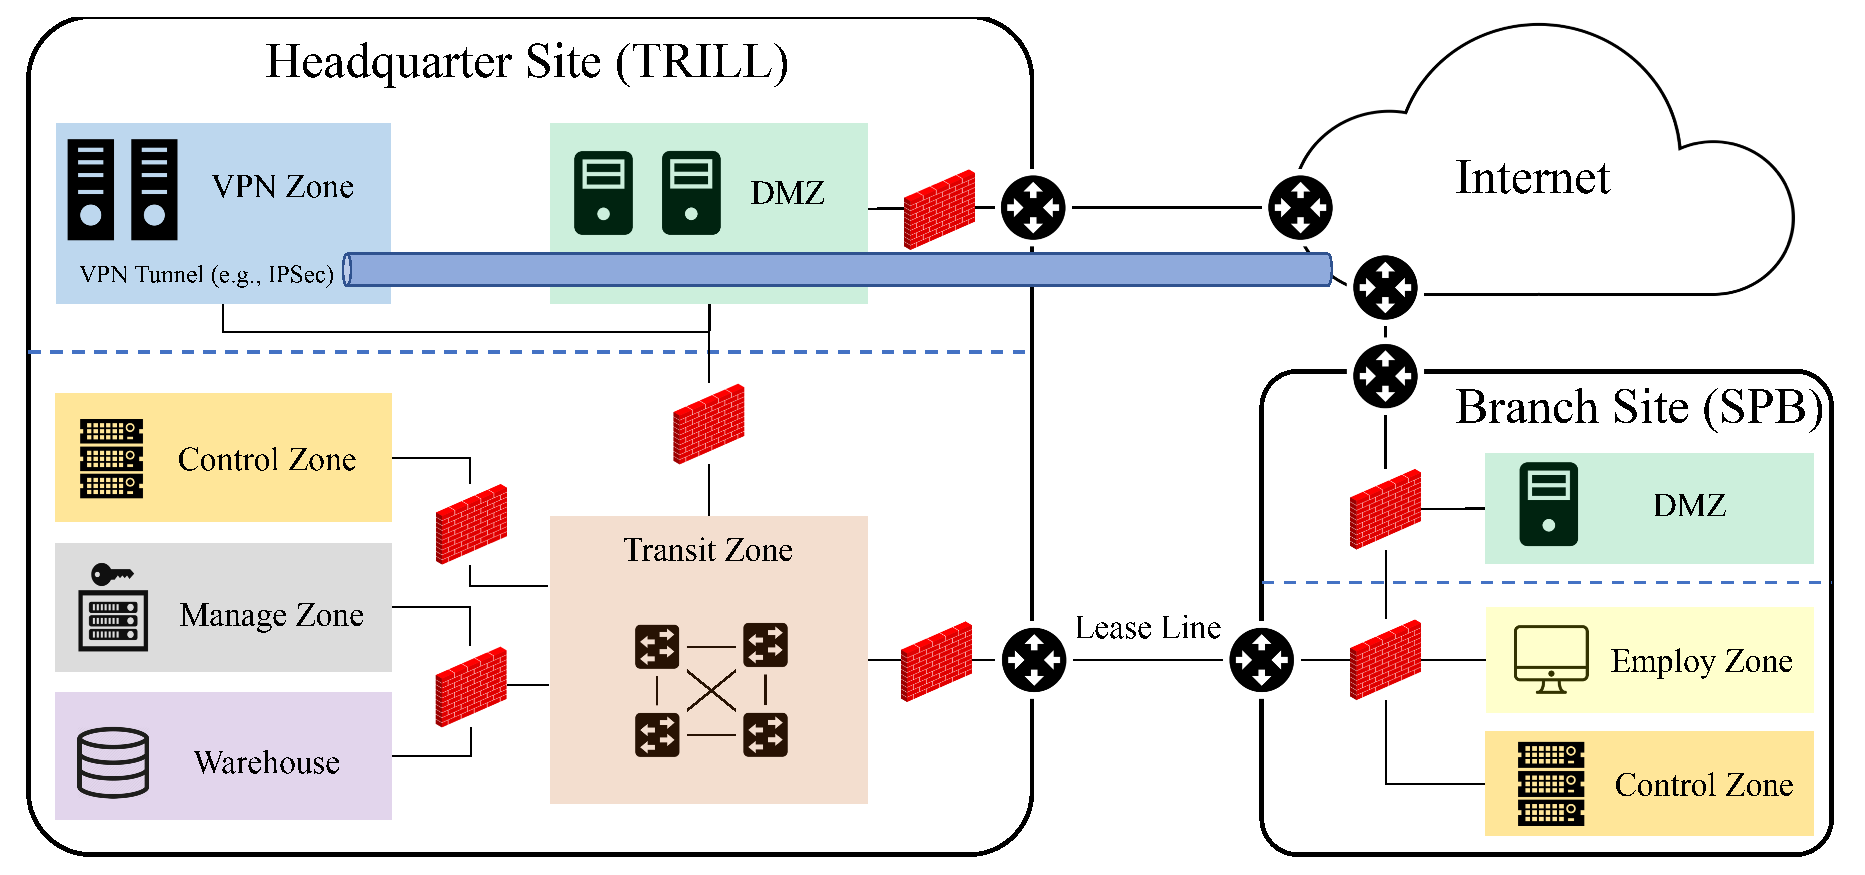
\includegraphics[width=.9\textwidth]{usecase.eps}
	\end{center}
	\caption{\textit{Network zoning use case for large enterprises. Network zones are
	realized with heavy use of security middleboxes (e.g., Firewalls).}}
	\label{fig:usecase}
\end{figure}

Most enterprise networks have embraced the notion of layered security classification,
that can be broadly split into intranet, extranet, and opennet~\cite{ramasamy2011towards}.
The opennet is the least trusted network (e.g., the Internet) which is an inhospitable region
where live threats exist, whereas the intranet is the most trusted network hosting
business-critical systems and sensitive information. Since the intranet has rigorous access
control mechanisms to protect information assets from exposure to the opennet, enterprises are
forced to operate another security layer (extranet, also known as demilitarized zone or DMZ) in between,
which exposes the publicly accessible services to the opennet, while reducing the attack surface of the intranet.

Over time, these layered network structures have become more sophisticated~\cite{obregon2015infrastructure}
due to extreme changes in network environments---diverse demands from customers, partners
and employees accessing enterprise networks with a variety of devices.
As a result, many enterprise networks
comprise a large number of zones defined by operational, organizational, and most
importantly security factors. Figure~\ref{fig:usecase} depicts a real-world use case for
network zones running on inter-domain level with multiple involved autonomous systems (ASes). They
can be categorized into three main types.

\paragraph{Intra-domain Zone Transfer}
% 1. direct transfer
% 2. through trasit zone
Within a local network, multiple devices such as servers, databases, and hosts are connected
through network switches. These devices are assigned with a unique IP address that belongs
to a logically isolated network zone. These zones commonly consist of multiple subnets,
often realized with a layer 2 virtualization technology (e.g., VLAN). Each zone is protected
by a set of security middleboxes, e.g., firewalls, intrusion-prevention systems (IPS),
and intrusion-detection systems (IDS), which enforce predefined security policies for all
traffic passing through.

To maintain the zone-based trust model, access permission to one zone is not considered to be
valid for other zones. That is, an entity must obtain access permissions from all zones on the
path when accessing a non-adjacent zone. This trust model however often complicates policy management
and enforcement, especially for large enterprise networks.
To resolve this complication, the current practice introduces the notion of a dedicated zone in which zone
transitions are handled, called Transit Zone.

\begin{figure}[htb]
	\begin{center}
		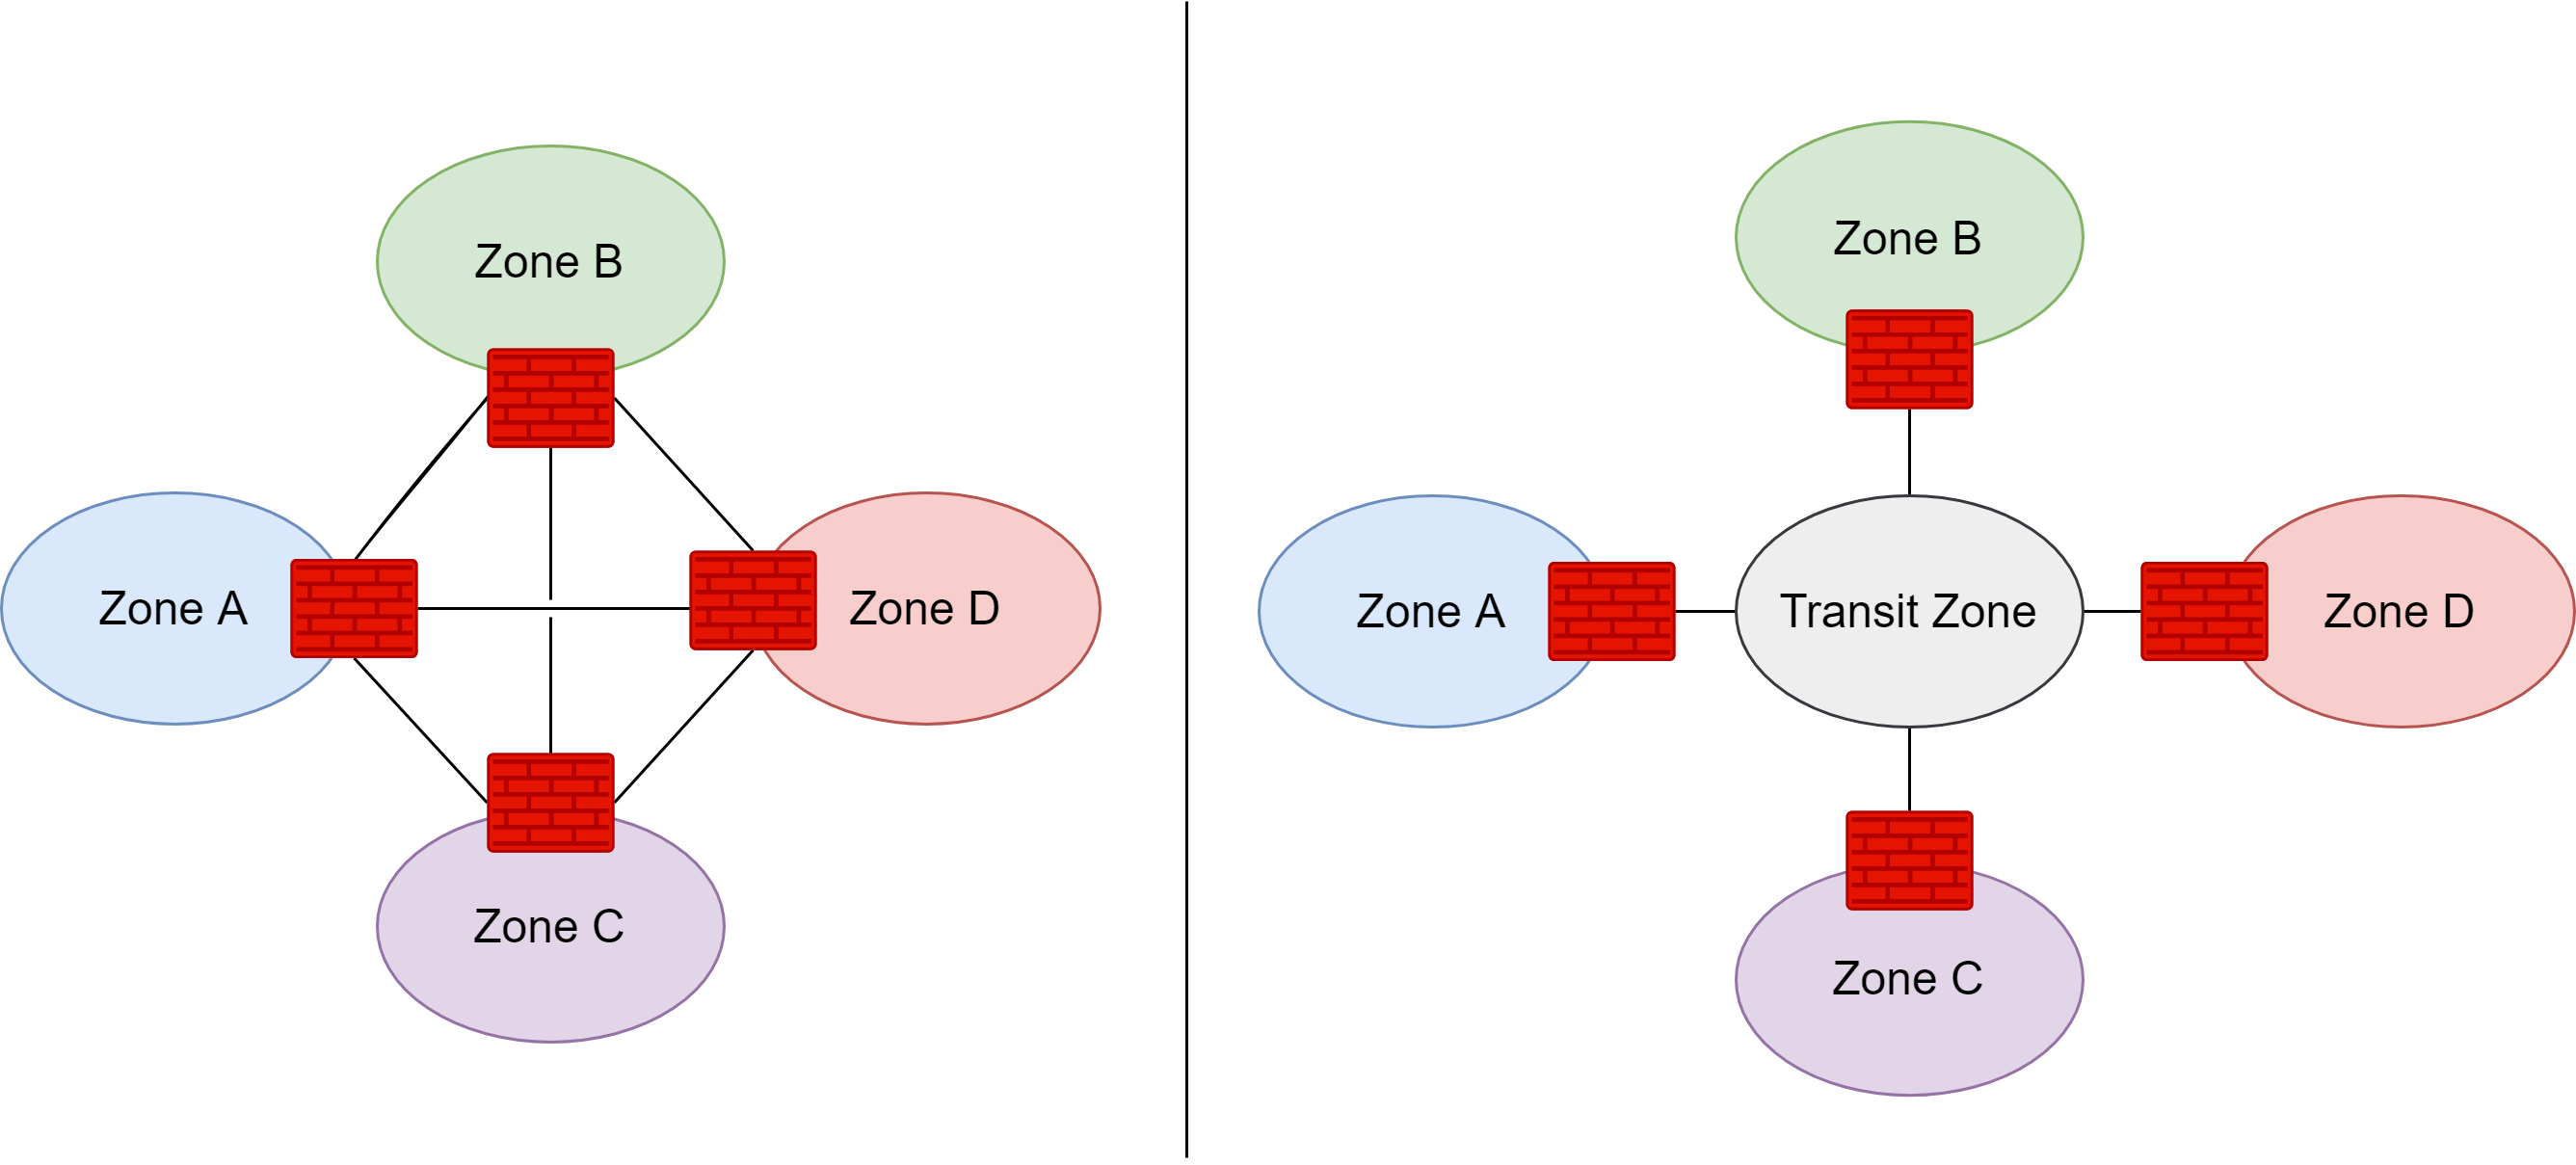
\includegraphics[width=.9\textwidth]{zone_layouts.png}
	\end{center}
	\caption{\textit{Two ways of structuring network zones. The use of a transit zone on the right side reduces
	the number of required links.}}
	\label{fig:zone_layout}
\end{figure}

A transit zone acts like a patch panel allowing zones to be interconnected without the need
of a dedicated link between each pair of zones (Figure~\ref{fig:zone_layout}).
The Transit zone sits in the middle of all
the other zones and mediates access between zones wishing to communicate with each other.
It is commonly comprised of only forwarding devices (e.g., switches), interconnecting the
attached zones via various ingress/egress points on which security middleboxes enforce the
security policies. In a nutshell, the Transit Zone reduces the depth of zone hierarchies and
thus simplifies the network zone design and management.

\paragraph{Inter-domain Zone Transfer}
% briding sites is expensive
To ensure that geographically distributed zones can securely communicate with each other,
enterprises employ various networking technologies. The most common choice is connecting
two remote sites with a physical private line, (e.g., layer 2 circuit). Enterprises
can lease these lines from Internet service providers and make use of them to bridge local
networks. However, purchasing private lines is costly and might come along
with trust issues towards the service provider.

An alternative is a virtual private
network (VPN). A VPN uses cryptographic primitives to create a virtual tunnel between two
local networks, preventing information leakage during transmission over the public Internet.
While the VPN technology ensures data confidentiality, typically yet another layer of overlay
protocols is required to achieve virtual separation of zones. The use of such overlay
protocols, however, has the disadvantage that all interconnected sites need to deploy the same
protocol since such protocols generally do not offer interoperability.

\paragraph{Traffic from the Internet}
% 1. normal customer
% 2. authorised user (employee)
% 3. attacker
Traffic not originating in cooperative (trusted) networks can be classified
into the following three types: i) public traffic, ii) authorized traffic, and iii)
malicious traffic. The first case covers normal customers who access the enterprise's
public services, e.g., Web servers. This traffic in general ends up at the demilitarized zone
(DMZ) hosting only public services that require exposure to Internet.
The second case refers to the traffic coming from temporarily authorized devices. For example,
a legitimate employee outside the enterprise's premises---working from home with a personal
device---may get a temporal permit to access restricted zones via VPN. The last
category comprises attack traffic which is to be filtered by the security middleboxes in the
frontline of defense.

% \begin{table}[t]
% % \caption{use case table. need to be merged with the fig_usecase}
% \label{tab:usecase}
% \centering
% \resizebox{0.48\textwidth}{!}{
% 	\begin{tabular}{*4{c}}
% 	\toprule
% 	& Between Zones & Through Transit Zone & Within Zone\\
% 	\midrule
% 	Inter-domain & \circled{1} $E_1 \leftrightarrow E_4$ 
% 	& \circled{2} $E_1 \leftrightarrow E_5$ & \circled{3} $E_1 \leftrightarrow E_2$\\
% 	Intra-domain & \circled{4} $E_5 \leftrightarrow E_6$ 
% 	& \circled{5} $E_3 \leftrightarrow E_4$ & \circled{6} $E_1 \leftrightarrow E_3$\\
% 	\bottomrule
% 	\end{tabular}
% }
% \end{table}

% \paragraph{Inter-domain Zone Transfer} % Case 1:
% \paragraph{Inter-domain Zone Transfer via Transit} % Case 2: 
% \paragraph{Inter-domain Communication within a Zone} % Case 3: 
% \paragraph{Local Zone Transfer} % Case 4: 
% \paragraph{Local Zone Transfer via Transit} % Case 5: 
% \paragraph{Local Communication within a Zone} % Case 6:
\cmnt{describe all 6 usecases here?}


\section{Challenges}
\label{sec:challenges}

\paragraph{Secure Zone Transfer}
Transmitting security-sensitive data between zones in different physical locations (e.g.,
data center to branch site) over the public Internet poses a challenge.
Security level information is lost in transit, requiring that the data is re-authenticated and
filtered again on the receiving site even though source and destination could be part of the
same logical zone.
Today's overlay protocols are often used to overcome the restriction of losing
security level information in transit. This, however, introduces new challenges: difficulties
in deployment per zone, computational overhead, and poor management scalability.

\paragraph{Interoperability}
Even if security-level information persists in transit, different zones might not be
built on the same internal protocols (e.g., SPB~\cite{ieee2012spb} vs Trill~\cite{rfc6325})
which makes it difficult for end systems in different zones to be able to seamlessly communicate
with each other.
% A new architecture therefore must be able to understand various network protocols and 
% interpret them into a local language that all target networks can understand. This means 
% that the interpretation should preserve the properties of an original protocol, such as 
% % layer-2 routing decisions. 
% virtual segmentation.
% % A flexible design for the architecture to easily embed new protocols also should be considered.
\cmnt{uncomment text, maybe rephrase}

\paragraph{Management Scalability}
In current local network zoning architectures, administration is being considered a tedious,
time-consuming, and labor-intensive task. For example, simply adding a new zone might
require existing policies to be thoroughly reviewed, updated, and re-distributed
to the local network entities. The management complexity dramatically increases in a
wide-area network (WAN) environment.
% For global orchestration across heterogeneous environments, a new architecture therefore
% must ensure management scalability. That is, network administrators should be able to easily extend 
% network zones in different physical locations and update policies that reflect these network
% changes, and be assured that no security loopholes were introduced.
\cmnt{uncomment text, maybe rephrase}

% easily scale up resources 





% \subsection{Industrial Perspectives}

% % \paragraph{Large Enterprise Networks}
% % In order to protect information technology assets, large enterprise networks are partitioned into disjoint segments which group together assets with the same security requirements and policies. These groups are referred to as zones. Zones define the network boundaries and their defense requirements by stating the entities populating the zones, the entry points into the zone as well as how traffic is monitored and filtered at these entry points. Oftentimes, these zones are realized by a (virtualized) separation at layer 2 with firewalls at higher levels governing data transfers between zones.
% Traditionally, enterprises used to consider three security layers for their network 
% environment: intranet, extranet and opennet~\cite{ramasamy2011towards}. The opennet is
% the least trusted network (e.g., the Internet) which is inhospitable region where live 
% threats exist, while the intranet is the most trusted network hosting business-critical 
% systems and sensitive information. Since the intranet has rigorous access controls to 
% protect the information assets from an exposure, enterprises put another security layer 
% (extranet) in between, that only exposes public services to opennet and thus reduces 
% attack surfaces. 
% As enterprises have recently witnessed extreme changes in network environment such as
% diverse demands from customers, partners and employees accessing their network with
% variety of devices, the enterprises employ more sophisticated network security 
% segmentation\cite{obregon2015infrastructure}, called security zones.
% Security zones constitute the logical grouping of one or more subnets that share the
% same security requirements and policies. 
% % Since security zoning is the foundation of 
% % network isolation criteria that must be upheld for secure business environements, 
% % the zone classification of information assets requires 

% Each security zone is identified with different level of trust, and every pair of zones 
% are defined with a namely trusted-untrusted relationship. 
% To realize the unidirectional trust model, firewalls are considered as the most viable
% technologies and widely used in the current practice. However, operating firewalls in 
% large enterprises is often challenging to network operators and security architects. The 
% access control for the security zones might be dynamic, and thus its requires a complex 
% management scheme to accommodate a myriad set of policies. While there are advanced 
% technologies such as virtual firewall~\cite{deng2015vnguard,bakker2016network} and Unified
% Threat Management (UTM)~\cite{qi2007towards}, that are newly designed for enforcement of 
% access control polices in extremely dynamic networks, security zone management and modeling 
% still remains to be evolved~\cite{ramasamy2011towards,gontarczyk2015blueprint}.

% Bridging geographically distant security zones can also be challenging. Oftentimes,
% security zones are created not only for security purpose but also because of geographical
% factors. Given that the security zones in distance should exchange information over
% public network (opennet as aforementioned), there might be a potential risk that the
% communication may expose security-sensitive information during transit. To mitigate
% such a threat, network operators leverage additional security control/mechanisms (e.g.,
% IPSec~\cite{rfc4301} and SSL VPN~\cite{sun2011advantages}) which ensure confidentiality
% and integrity of the transmission over the untrusted network by encrypting the data with
% securely shared cryptographic keys. Nonetheless, the technologies might bring new challenges
% such as management scalability~\cite{felsch2018dangers} and compatibility to the secure 
% isolation~\cite{liu2008collaborative}.

% % \paragraph{Cloud Computing (LaaS, PaaS, SaaS)}
% The cloud computing environment is a good representative example that depicts such practical 
% challenges. Cloud-based service providers operate large multi-tenant data centers which 
% have to scale to customers needs. To achieve this scalability while at the same time staying
% cost efficient cloud providers make heavy use of virtualization techniques. This environment 
% challenges operators with providing secure segmentation between tenants as multiple tenants 
% are using the same physical machines and network. In addition, given that the cloud 
% environments comprise geographically distributed data centers, providing secure communication 
% channels between security zones while upholding a constant view of the security policies
% under the dynamic zone migration is another hill to climb. Now, we derive main challenges 
% we confront in this research with case study.
% % Legal requirements need to be respected. Furthermore, an optimal solution needs to be highly 
% % flexible as the number of assigned resources for a given customer can change frequently.



% % \paragraph{Edge Computing}
% % With the rise of mobile devices and Internet of Things (IoT) new types of data intensive, time
% sensitive applications are emerging. (e.g. VR/AR) However, since these devices are also required to
% be low power they cannot do these heavy computations themselves. Cloud computing can be used to
% offload the work to centralized data centers. However, this causes new challenges. Often, the latency
% between devices and the cloud is too high and therefore not well suited for real-time applications.
% Additionally, a large number of devices means that a centralized infrastructure can get saturated by
% big traffic flows. One widely used solution to this problem is Edge Computing which puts nodes handling
% the computation close to end devices.
 % Background Theory 
\chapter{Related Work}
\label{related}

\cmnt{move to bottom?}

% \paragraph{Security Zoning}
% During stacking our knowledge of security zoning, we noticed that there is a limited number of academic research on network zoning architecture while considerable research is underway in the industry regarding access management and system design. 
% firewall architecture 
% 1. standalone
% 2. distributed
% 3. virtualized
% 4. colaborative 
The majority of literature in network zoning has focused on security enforcement architecture using middleboxes such as firewalls, IPS, and IDS.
Conventional security middleboxes define restricted zones and filter unwanted traffic at the entry points of protected zones~\cite{cheswick1994firewalls}. 
As information systems and the corresponding network functions got more complicated, the notion of distributed security systems has been introduced in the late 1990's~\cite{bellovin1999distributed}.
Early approaches to protect only internal information systems from external threats have further evolved to mitigate sophisticated threats, for example insider attacks, rule tampering, application-level proxies, and denial-of-service attacks~\cite{markham2001security}.
Later, with emerging network virtualization technologies and cloud computing environments, virtual firewalls and collaborative security enforcement kept getting attention from both academia and the industry~\cite{liu2008collaborative,yu2017psi}. 

Despite numerous research efforts, network zoning using security middleboxes has issues with respect to performance---the iMIX throughput degrades by 40 - 75\% on commodity products~\cite{juniper2020comparison}---and misconfigurations~\cite{fayaz2016buzz,tschaen2016sfc,yuan2020netsmc}. 
With \name, we address these challenges by leveraging a cryptographic-based policy enforcement and centralized policy orchestration, achieving scalable, effective, and cost-efficient network zoning.

% Zoning is orthogonal with all the concepts.
% Zoning is a fundamental piece. Zoning need to be done first in scale passion to decide which node can communicate which other nodes, then put firewalls, ids, and ips.
% All the the previous technologies is for single zone. Given the complexity, 

% \paragraph{Network Segmentation and Isolation}
Network isolation through network segmentation is another essential element of network zoning. 
To logically segment the physical network, network virtualization technologies are heavily used in today's Internet, in particular large enterprise networks and cloud computing environments.
VLAN~\cite{ieee2018vlan} is the most frequently used network segmentation technique.
It logically segments a physical LAN into up to 4094 virtual LANs by tagging the layer 2 header with a unique VLAN identifier (VID).
Later, Virtual eXtensible LAN (VXLAN)~\cite{rfc7348} has been introduced for better scalability; it expands the number of virtual LANs to up to 16 million by leveraging a 24-bit identifier.
SPB~\cite{ieee2012spb} and Trill~\cite{rfc6325,rfc7176} are layer 2 routing protocols enabling multi-path communication among virtual LANs within the same physical LAN. 
Although security is an important property when it comes to network segmentation, it unfortunately
has often not been treated as a major concern. Systems lack protection for segment membership and access control.
To isolate each segment, use of a large number of security middleboxes is necessary, thus increasing operational costs and management complexity. 

SVLAN~\cite{kwon2020svlan} is an architecture enhancing security in network isolation by enforcing the receiver's consent towards incoming traffic. 
SVLAN is the closest work related to \name, but there are three major differences.
First, \name decouples policy establishment and enforcement. In SVLAN, the authorization delegate (i.e., controller) is responsible for establishing basic reachability policies and issuing authorization tokens to enforce the policies.
The single trust model requires additional latency to fetch the authorization token for a new flow.
In contrast, \name leaves the policy enforcement to the data-plane, reducing overhead.
Second, \name provides data confidentiality.
SVLAN focuses on bridging layer 2 networks and thus leaves higher-layer protocols responsible for communication security. 
Lastly, \name is compatible with various Internet architectures, whereas SVLAN is relying on segment routing~\cite{rfc8402,rfc8660}. 
Although segment routing is an emerging technology, yet it is not completely supported especially for collaborative wide-area networks, and thus constrains deployability.

 % Discussion of Related Work
\chapter{Overview}
\label{overview}

This chapter provides an overview of \name. We first elaborate the fundamental goals
of this research, along with requirements, and design choices (\S\ref{sec:design}).
We then outline \name including a brief introduction of each component and their
workflow (\S\ref{sec:overview}). Finally, we describe our threat model
(\S\ref{sec:threatmodel}) and state our assumptions (\S\ref{sec:assumptions}).

\section{Design Principles}
\label{sec:design}

\paragraph{Goal}
The fundamental goal of this work is to build an architecture that combines local
network zoning and inter-domain routing with regard to secure zone transfers, lightweight protocol interoperability,
and incremental deployability---thereby enabling secure,
scalable, and flexible network zoning on a global scale. That is, an administration
domain expresses zone definitions and corresponding zone transfer rules, and
deploys the policies to distributed network entities. These policies force the
network to only forward authorized packets protected by cryptographically
secured authenticators, ensuring secure and sustainable zone-to-zone communication.

\paragraph{Desired Properties}
We consider the following properties to achieve this goal.

\begin{itemize}
	% \item Strong security guarantee: the zone transfer protocol applies strong
	% cryptography primitives, such that no security sensitive information is exposed 
	% while the data is being transmitted via the public Internet. 
	\item Data confidentiality: through a constructive approach, the zone transfer
	      protocol ensures that no information
	      is exposed while being transmitted via the public Internet.
	\item Management scalability: logically centralized orchestration empowers
	      network administrators to easily migrate network topologies, update policies and
	      mirror abstract network zones into the real network.
	      % \item Practicality: the modern cryptographic primitives that we use are 
	      % lightweight, such that they do not introduce severe performance overheads in terms of 
	      % latency, bandwidth, and operational costs.
	\item Efficiency: the cryptographic primitives introduce only minor performance
	      overhead in terms of latency, bandwidth, and operational costs.
	\item Deployability: the \name architecture requires minimal changes to the
	      existing network infrastructure in order to achieve compatibility. Furthermore,
	      firewalls and VPN devices
	      at each entry point of every zone can be replaced with one \name gateway, saving
	      operational costs for the same level of network security.
\end{itemize}


\paragraph{Design Choices}
% We design \name working with mature technologies that are well embraced in 
% modern the Internet environment, such that our architecture keeps its practicality 
% and deployability. In particular, the following design choices are considered:
We design \name working with mature technologies that are embraced in modern enterprise
environments. In particular, the following design choices are made:

\begin{itemize}
	\item Network programmability is realized with the concept of a logically centralized
	      controller (e.g., SDN), preserving management flexibility and scalability.
	\item Asymmetric cryptography is used for core operations where source
	      authenticity is critical (e.g., symmetric key exchange).
	\item Symmetric cryptography is used for the rest of the data
	      transmission, ensuring efficient packet processing.
\end{itemize}

\begin{figure}[htb]
	\begin{center}
		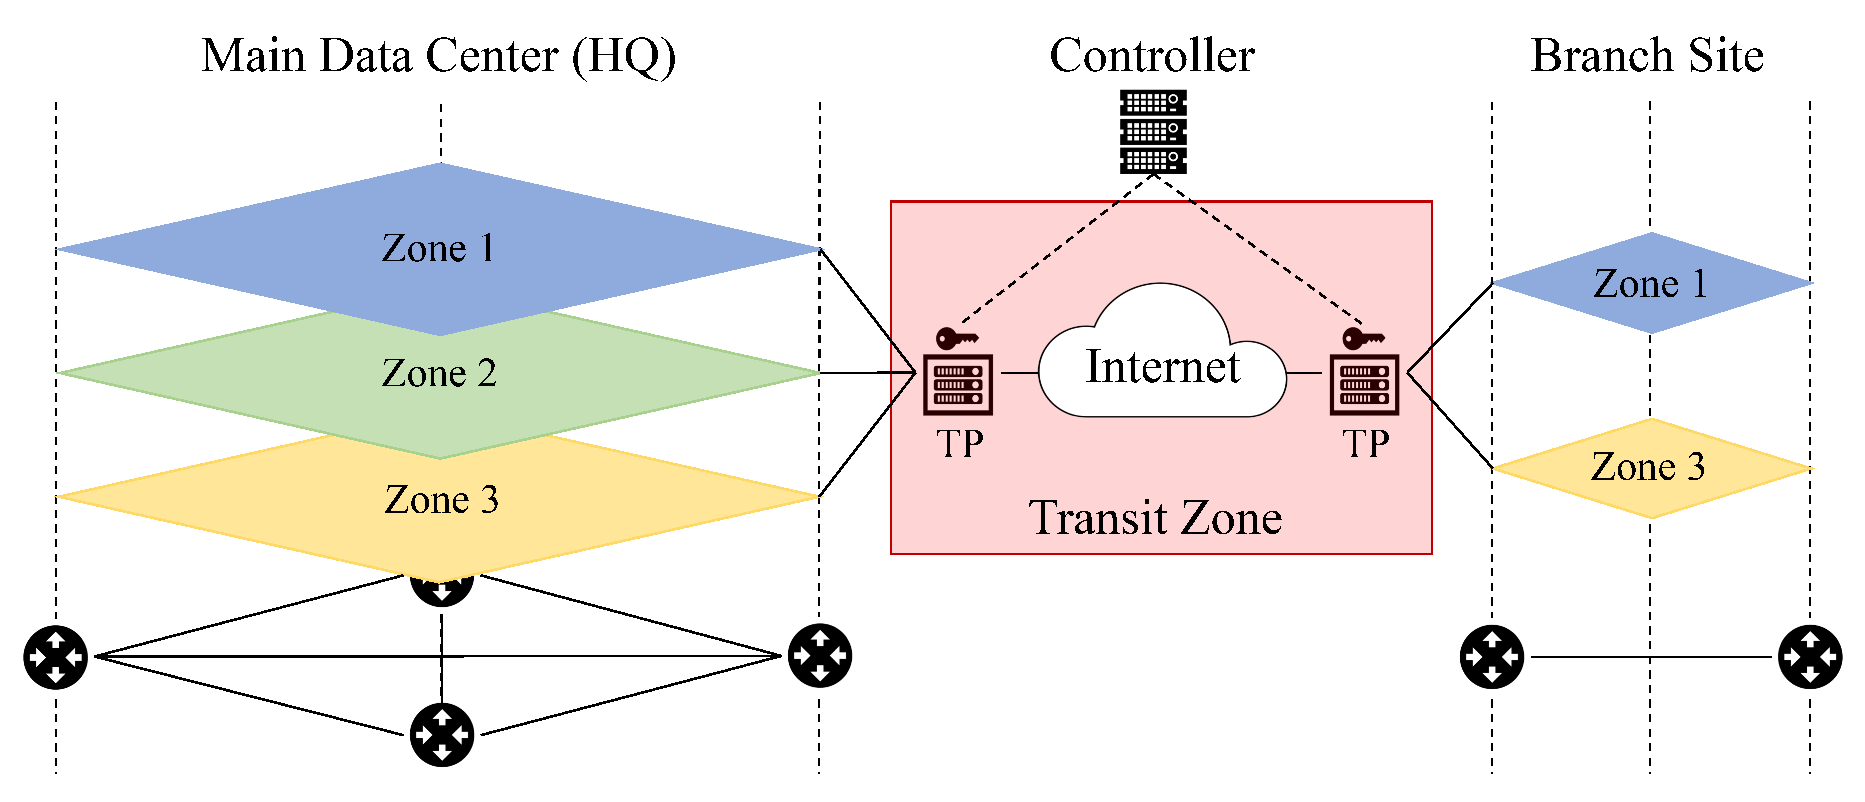
\includegraphics[width=.9\textwidth]{overview.eps}
	\end{center}
	\caption{An overview of \name architecture. The inter-domain transit zone interconnects physically
	and logically distributed network zones with unified security policy enforcement.}
	\label{fig:overview}
\end{figure}

\section{\name Overview}
\label{sec:overview}

\paragraph{Entities in \name}

\begin{floatingfigure}[r]{0.5\textwidth}
	\centering
	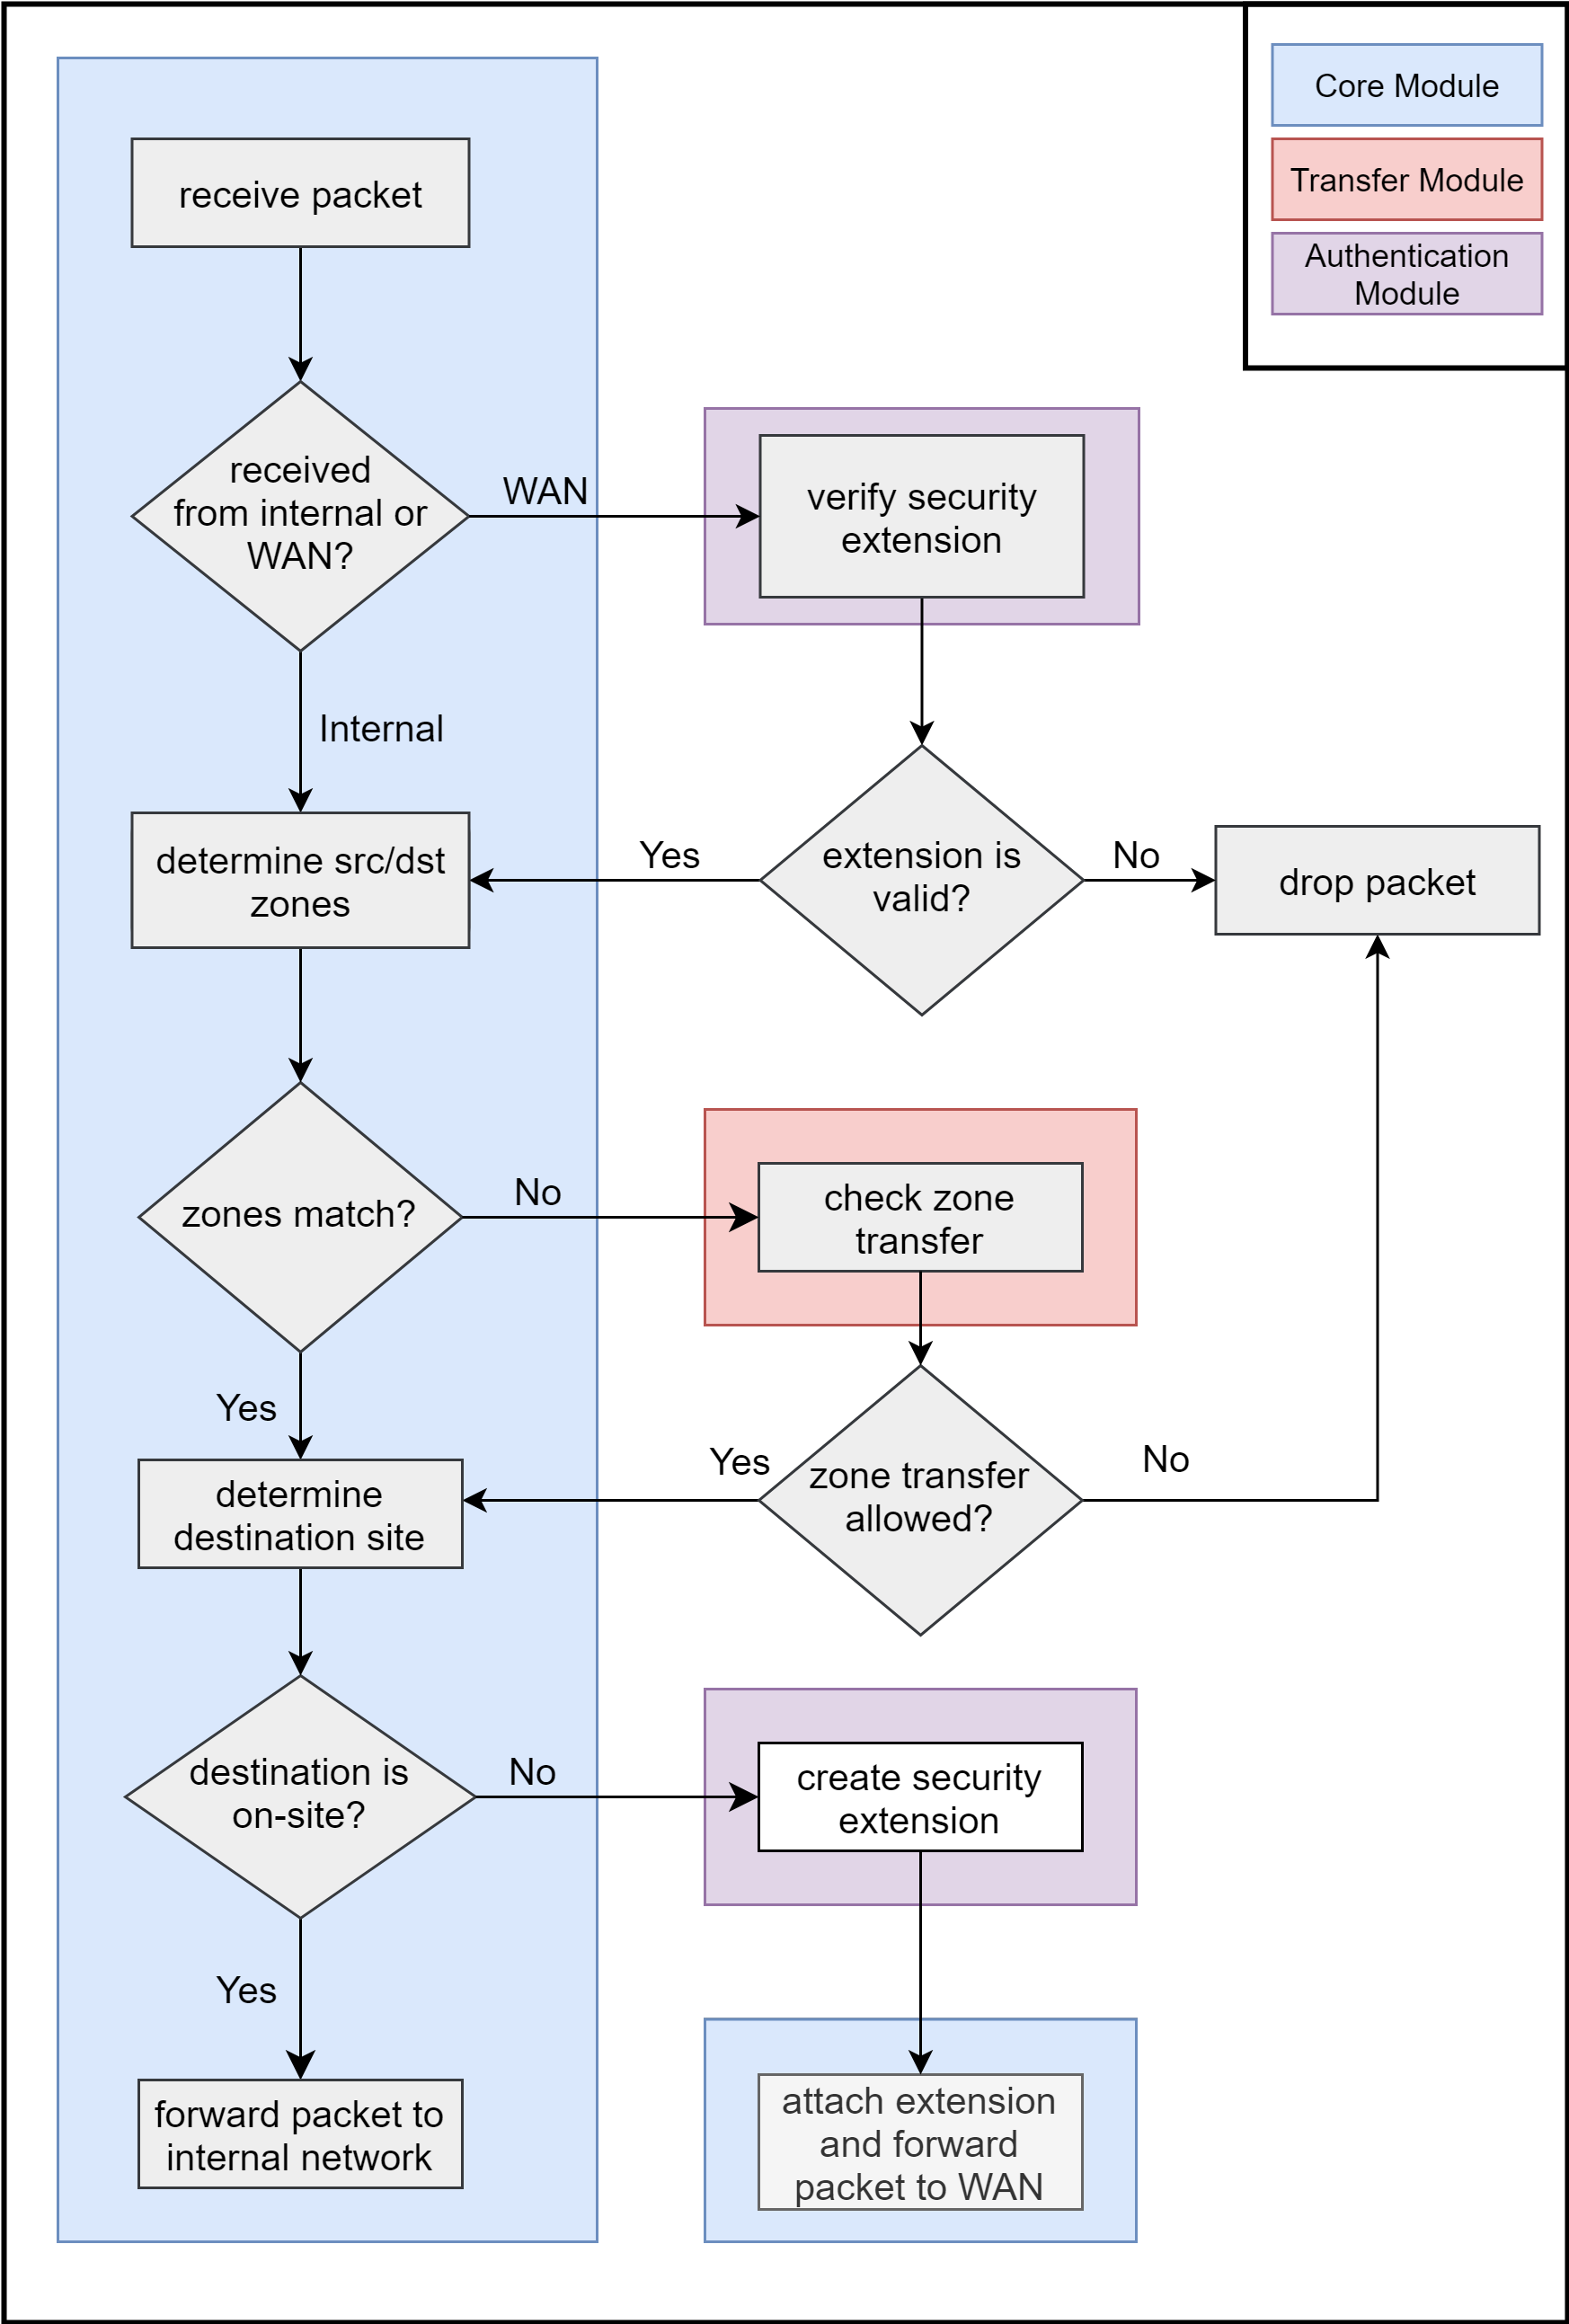
\includegraphics[width=.49\linewidth]{tp_controlflow.png}
	\caption{Control flow of the Zone Translation Point}
	\label{archi:flow}
\end{floatingfigure}

Figure~\ref{fig:overview} illustrates an overview of \name.
Different branch sites of an enterprise are interconnected over a WAN (\eg the Internet). Each site
contains multiple, logically separated zones connected to the single Zone
Translation Point (\tp) at the corresponding site. The \tp is a designated gateway
for zone transfers, operating on layer 3 and interconnecting all zones at a given
site of the enterprise network. All the traffic towards either internal network or
WAN, therefore, passes through the \tp. Note that \tps are the endpoints
of our architecture, meaning that everything beyond that point should not be
modified for ease of deployment and to ensure compatibility with the modern enterprise
environments.

The main task of \tps is twofold:
first, they ensure that traffic adheres to a set of allowed zone transitions. For
a packet originating in a zone and destined for another zone, the transition must be
explicitly allowed by a policy. Second, \tps enable communication across the WAN without
losing previously established security information. To this end, \tps embed a tag
with cryptographically secured zone information into packets before they leave the
internal network. Furthermore, \tps act as endpoints hiding sensitive information,
such as internal addresses and the respective zone binding, from external entities.
We also note that, for a case where zones with the same security requirements and
functionality are distributed over multiple branch sites (e.g., Zone 1 and 3 in
Figure~\ref{fig:overview}),
we consider them as the same logical zone (e.g., the same zone identifier). We call
this concept zone extension which is not subject to zone authorization.

A logically centralized controller orchestrates the \tps. The controller is owned
by a single administration domain, and thus the owner of the controller owns all
the zones behind the \tps. The controller provides its owner a management interface
in which the owner designs an outline of zone structure and transfer policies. The
explicit network configuration is then distributed to the \tps via a secure control
channel to enforce the configuration at the individual premises.

\paragraph{Communication Flow}

\name enables secure zone transfers over WAN as follows:

\begin{enumerate}
	\item Network administrators first establish an IP-zone map and their transfer
	      policies, which represents a virtual network configuration that explicitly
	      specifies reachability, and upload them to the logically centralized
	      controller.
	\item Each pair of \tps exchanges symmetric keys to establish a secure tunnel.
	      The key is being updated frequently through a state-of-art key management and
	      distribution system that protects the secrecy of the zone transfer from
	      being exposed to the public while ensuring high-speed data transmission.
	\item The on-site \tp inspects all the packets to be transmitted to another zone.
	      The \tp acquires the corresponding zone transfer policy from the controller
	      and verifies if the transmission is authorized.
	\item If a packet is authorized, the \tp looks up the respective end-point \tp,
	      encrypts the packet along with the corresponding zone transfer information,
	      and forwards it across the WAN. Otherwise, the packet is dropped.
	\item The remote-site \tp then decrypts the packet and forwards it according to
	      the enclosed zone transfer information. The receiving \tp could also verify
	      the validity of the packet transmission if desired.
\end{enumerate}

Figure~\ref{archi:flow} shows the control flow of a \tp.

\section{Threat Model}
\label{sec:threatmodel}
We consider a threat model in which attackers reside either on-premise (i.e., compromised
end hosts) or are located
outside of the cooperative networks. The goal of attackers is to access unauthorized zones
to exfiltrate information assets, or disrupt networks and services. To achieve this goal,
attackers can use the following strategies:

% \paragraph{Reconnaissance}
% % Attackers can observe or collect legitimate network traffic at "Checkpoint 
% % Charlie"---aggregation points where the zone transfer packets traverse---to map the
% % pairs of hosts and their corresponding security policies. For instance, tapping the
% % wire near entry points of enterprise networks is feasible. 
% Attackers can observe or collect legitimate network traffic at aggregation points through 
% which the zone transfer packets traverse, to map the
% pairs of hosts and their corresponding security policies. For instance, by eavesdropping
% near entry points of enterprise networks. 

\paragraph{Unauthorized Access}
Attackers may disguise as authorized entities to blind the security middleboxes and
access restricted zones.
% We have witnessed that impersonating other network entities 
% is a common attack scheme in many network systems. \ml{Is there something to reference?} 
A more sophisticated attack is to override security systems by directly injecting
tampered policies.

\paragraph{Denial-of-Service}
Here, the goal is to disrupt the target networks or services. Attackers can sabotage the core network
systems, for example, by flooding security middleboxes that perform deep packet inspection.
This might then lead to network performance degradation, causing
denial-of-service for legitimate clients.

% \paragraph{Exfiltration}
% Sensitive and business-critical data is stolen and forwarded to a remote server on the
% attacker's premises. In most cases, the data is stored in the restricted zones with 
% the highest level of trust---establishing a communication channel from highly trusted
% zones to a low-level zone is commonly not constrained---attackers can easily exfiltrate
% the highly valuable information assets. \claude{I don't understand this scenario. How does the attacker get access to a high security zone?} \jk{This is an attacker model after succeeding 
% infiltration to the high secure zone. Nonetheless, we'd better not to describe this anyway.}

% In our threat model, we assume that components of \name (i.e., \tps and controllers) 
% are resilient against compromise attacks, and therefore trustworthy.


\section{Assumptions}
\label{sec:assumptions}

\paragraph{Public Key Infrastructure}
A given enterprise network has a public key infrastructure (PKI). That is, the enterprise
creates a trust model for its network infrastructure, acts as a trusted certificate authority
(CA), and issues certificates for the core systems. Entities can retrieve and verify the
public keys of the core systems. There are open source projects, such as \fnurl{EJBCA}{https://svn.cesecore.eu/svn/ejbca/trunk/ejbca/} and \fnurl{OpenXPKI}{https://github.com/openxpki/openxpki/}, available for setting up enterprise-grade PKIs.

\paragraph{Secure Cryptography}
Cryptographic primitives we use in \name are secure; authenticity, integrity, and
confidentiality remain intact unless the cryptographic keys are exposed.

\paragraph{Time Synchronization}
Core entities within the cooperative network have loosely synchronized system clocks with a
precision of seconds (e.g., network time protocol achieves a precision of tens of milliseconds).
Time synchronization is mainly used to constrain the validity of cryptographic keys.

\paragraph{Sole Administration}
A network has a sole administration domain (e.g., enterprise) which has full control over
the network architecture and security policy. To access the network, collaborators
must obey this policy.

\chapter{Architecture}
\label{arch}

In this section, we present the \name architecture and the underlying protocols in detail. 
Later, we describe our key-establishment system that enables rapid key derivation 
and distribution in large networks. 

\section{\name Bootstrapping}
\label{sec:bootstrapping}

The bootstrapping procedure is performed when a new zone or a new remote site 
(a group of zones along with a \tp) joins the network. 

\paragraph{Zoning Policy} % about zone itself 
A network zone is a logical concept, a group of network segments. A widely adopted 
segmentation technology is Virtual Lan (VLAN) which is used to separate networks on
layer~2. For example, zones are made up of multiple disjoint layer~2 networks
all identified by their corresponding VLAN ID (VID). A VID can be reused as long
as networks using the same VID are kept separate.

In \name, IP subnets correspond to exactly one network zone, such that the zone
a host belongs to can be identified by the host IP address. The same private
address spaces can be a part of different zones, and they are distinguishable by a
combination of their ASN (autonomous system number) and IP subnet. 
% \ml{Where does the ASN come from here? Couldn't the same private address space be used on different sites which are located in the same AS?} 
Consequently, each zone is defined as:
\noindent 
\begin{subequations}
	\begin{align}
		ASN \times IPsubnet & \mapsto VID,    \\
		\tp \times VID      & \mapsto zoneID. 
	\end{align}
	\label{eq:zoning}
\end{subequations}
\noindent 
% \claude{VID $\subseteq$ \{ASN: IPsubnet\}}
% \claude{ZoneID $\subseteq$ \{TP : VID\}}
% \claude{I was again thinking about this notation. I feel like the element notation conveys the wrong idea that one VID/ZoneID is limited to exactly one ASN:IP or TP:VID respectively. Maybe the subset ($\subseteq$) relation is more suitable here.}
% \ml{Is the VID supposed to actually \emph{consist} of ASN and IPSubnet (in terms of the bit representation) or rather \emph{refer} to (a set of) ASN:IPSubnets? In the latter case, a relation or function from VIDs to the combination of ASN:IPSubnets might be the most appropriate notation (same holds for ZoneIDs).}
% \ml{When typesetting names in math mode it is preferred to sourround them by ``mathit'' or ``text'' (whichever is preferred), as otherwise individual letters are understood as individual variables and spacing is suboptimal.}
The way zones are described here corresponds to how enterprises typically
segment their networks today, upholding backward compatibility and consequently
deployability. Furthermore, \name does not depend on the specific layer~2 protocols used 
at each site. 

Every zone is under one ownership, e.g., company A. In case multiple companies
want to collaborate by sharing certain network zones, it is one company that 
creates and owns the zones and the other companies simply join the network.

\paragraph{Zone Transfer Policy}
To allow network operators to explicitly express their zone transfer policies, we 
consider both denylist and allowlist-based policy establishment. 
% \ml{There are currently some suggestions of replacing blacklist/whitelist by \{block,deny\}list/allowlist.} 
This is a
mature approach commonly used in modern network management systems, enabling flexible
and agile orchestration of complex networking policies. The following depicts the
zone transfer policy format:
\noindent 
\begin{equation}
	<zone_{dst}, zone_{src}> \\ 
	\Rightarrow~<action, priority, time>
	\label{eq:policy}
\end{equation}
\noindent 
$action$ determines the corresponding action for the given source and destination
zone pair, e.g., \texttt{forwarding}, \texttt{drop}, and \texttt{established}. Similar
to \textit{iptables} rules, \texttt{forwarding} would allow any incoming packets from
the source zone whereas \texttt{drop} discards all traffic. \texttt{established} allows
incoming traffic for all established connections. 

In an event of conflict where $zone_{src}$ has different
access authorizations for the $zone_{dst}$, the conflict can be resolved by the field 
of $priority$. That is, a policy with a higher priority would be enforced in the zone 
If conflicting policies have the same priority, the most recently established policy 
according to $time$ would be enforced.

% In principle, VLAN is an layer~2 technology, running on a local network. To allow
% such VLANs 

\paragraph{Translation Point Initialization} % about tp
A \tp is initialized when a new remote site opens, prior to any communication between
zones. The initialization process has mainly two goals: i) bootstrap a secure channel 
with its controller to exchange control-plane messages, and ii) establish secure tunnels 
with other \tps for data transmission.
% A \tp is initialized when a new remote site opens, prior to any communication between
% zones. The initialization process has mainly three goals: i) bootstrap a secure channel 
% with its controller to exchange control-plane messages, ii) synchronize with the controller
% in terms of zone creation and translation policies, and iii) establish secure tunnels with
% other \tps for data transmission.

Upon bootstrap, a \tp performs a \textit{client-authenticated TLS handshake} with its 
controller in order to exchange their certificate, and agree on a cipher suite and compression
method. The \tp finds the corresponding address in its configuration file. This means 
that, prior to first use, there needs to be an out-of-band setup where the \tp is 
configured. This can either be done by the owner of the controller shipping a pre-configured 
machine to the new remote location or by the remote location setting up a machine and 
granting the controller owner management access to the given machine. Bootstraping \tps 
with multiple controllers will be described in~\S\ref{sec:distributedcontroller} with
practical considerations such as controller discovery, \tp migration, and policy consistency.

The controller synchronizes with \tps to keep their list of other \tps in the network 
up-to-date. To this end, the controller frequently pushes a list of relevant \tps with 
which a \tp can communicate.
% \claude{actually only the relevant subset of \tps is needed} 
% \jk{How does controller know the "relevant" \tps?}. 
This can be done either regularly (e.g., on a daily basis) or occasionally
(e.g., when a new \tp joins the network).
\tps then establish a secure channel with new \tps. To prevent \tps from using a stale \tp list,
the shared \tp list is associated with a time to live (TTL) value. 
% \claude{what does behind mean here? Still confused by this point? Does it mean in order to prevent TPs which were left behind by the synchronization from trying to fetch keys from stale TPs we associate the list with a timeout? }

For ``\textit{trust-even-before-first-use}'', 
% \ml{to me, this term refers to implicitly trusting the communication partner at first use. This is not what is used here where the entities explicitly authenticate each other.} 
the \tps and controller must be able to verify each 
other, preventing: i) a legitimate controller pushing information to an unauthorized \tp, 
and ii) a legitimate \tp connecting to a bogus controller or \tp under an attacker's control.
We ensure source authenticity of the \name entities by leveraging PKI-based identities.
The main idea behind the source authenticity is that all the \tps and controllers obtain
digital certificates for their IP address from a public key infrastructure (PKI). The owner 
of the entities (e.g., an enterprise) is a certificate authority, and issues the certificates
before an entity bootstraps. To this end, we consider well-established practices, e.g.,
the Resource Public Key Infrastructure (RPKI)~\cite{rfc7115,rfc6810}.
%  in the current Internet 
% or the SCION control-plane PKI in SCION future Internet architecture~\cite{Perrig2017}.
% \ml{At this point it is unclear what this has to do with SCION.}

% Upon bootstrapping, a \tp perform the \textit{client-authenticated TLS handshake} with its
% controller. That is, the \tp and controller exchange their certificate, agree on a cipher
% suite and compression method. Once the secure channel establishes, the \tp sends the 
% controller a \texttt{ZoneSync} request as:

% \begin{equation*}
% TP \rightarrow C: \Rightarrow~<action, priority, time>.
% \end{equation*}


\section{Protocol Description}
\label{sec:protocol}

Now, we describe how two end hosts within different remote sites are able to communicate. 
Figure~\ref{fig:protocol} illustrates a protocol level design including authorization,
forwarding, and verification. A detailed header design follows.

\begin{figure}[t]
	\begin{center}
		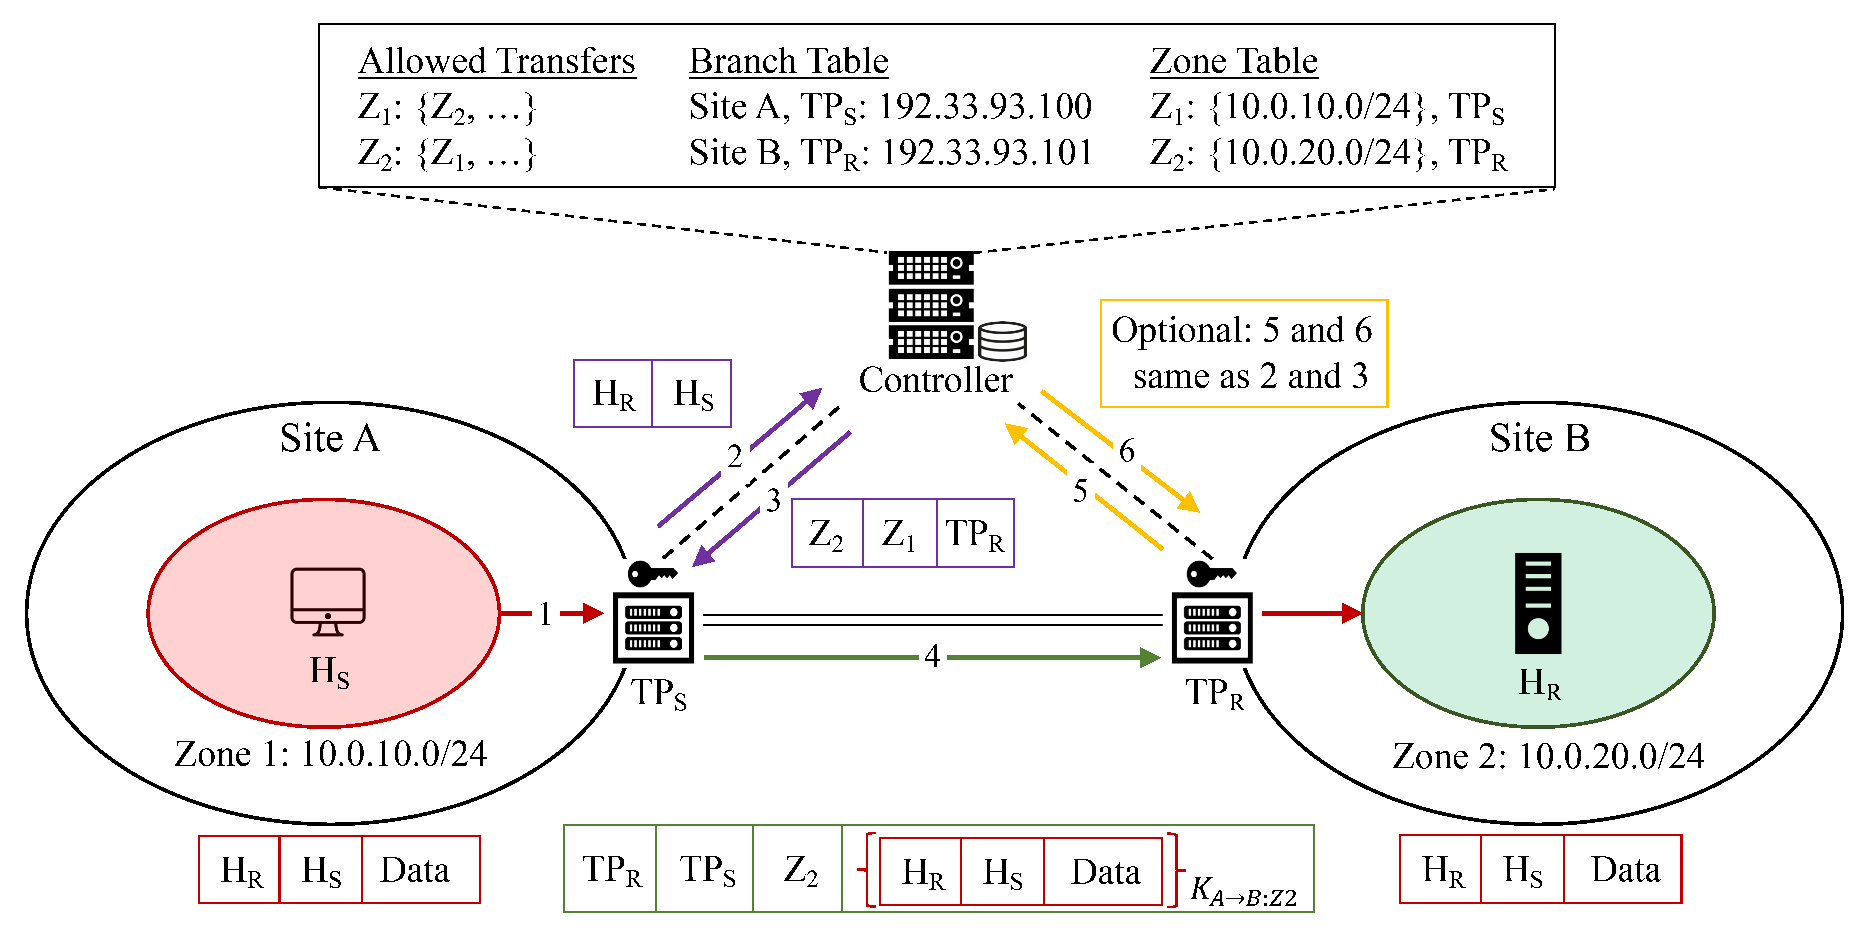
\includegraphics[width=.9\textwidth]{protocol.eps}
	\end{center}
	\caption{Protocol details for data forwarding. The controller frequently updates \tps 
	with the latest zone transfer policies.}
	
	\label{fig:protocol}
\end{figure}

% \paragraph{Zone Migration}

\paragraph{Zone Transfer Authorization}
End hosts behind a \tp operate as they normally would when they reside in a local network connected to a commodity gateway. That is, without any acknowledgment on network changes, a sender $H_S$ 
sends a packet to the receiver $H_R$. If $H_S$ and $H_R$ are residents of the same subnet 
(namely the same zone), the packet will be directly steered to the destination by the local 
forwarding devices. If $H_R$ is in a different subnet (or a remote site) however, the packet
is first delivered to $\tp_S$ since $\tp_S$ is the gateway of $H_S$. % (\tcircled{1}). 

To determine if the packet is allowed to be forwarded to the given destination zone $B$, $\tp_S$
needs an explicit zone-transfer policy for the given source and destination pair. Ideally, 
the policy is cached in the $\tp_S$'s zone transfer table. In case the cache misses, $\tp_S$ 
acquires the policy from the controller $C$ as follows:

\begin{enumerate}
	\item $\tp_S$ requests a zone-transfer policy from $C$:
	      \begin{equation}
	      	\tp_S \rightarrow C : H_R~|~H_S
	      	\label{eq:authreq}
	      \end{equation}
	\item $C$ replies with the zone-transfer policy:
	      \begin{equation}
	      	C \rightarrow \tp_S : \\
	      	Z_R~|~Z_S~|~rule~|~\tp_R~|~ExpTime
	      	\label{eq:authrep}
	      \end{equation}
\end{enumerate}

The controller consults the zone-transfer policy to see if the packet is allowed to be forwarded
to $H_R$, more specifically to destination zone $Z_B$. To this end, the controller 
first checks the corresponding zone information (Equation~\ref{eq:zoning}), and matches 
it with the zone transfer rules (Equation~\ref{eq:policy}). The authorization result is
then delivered to the requesting \tp along with the corresponding source and destination 
zone identifiers ($Z_R$ and $Z_S$ respectively), the destination \tp address 
($\tp_R$), and the expiration time ($ExpTime$) for the policy. $ExpTime$ can be an arbitrary
number, but we consider it to be a small number used for policy freshness.

\paragraph{Data Forwarding}
The \tp discards the packet (Host Unreachable) if $rule=$ \texttt{drop}. Otherwise, 
the \tp looks up its routing table and transmits the packet. There exist two types of 
zone transfer cases: one for local (same-site) zone transfers and another for remote zone 
transfers as addressed in \S\ref{sec:casestudy}. For the local zone transfer, the \tp 
simply rewrites the Ethernet header by following the local layer~2 protocol, and 
forwards it through a corresponding interface. Since the local network is assumed to
be trustworthy, no additional packet processing is necessary apart from the authorization.

For the remote zone transfer, the \tp is responsible for the secure transmission of the
packet towards the destination \tp. Recall that it is important for the inter-domain 
zone transfer packet to keep confidentiality and integrity in transmission. We therefore 
leverage the notion of secure tunneling, i.e., the IPSec tunnel mode~\cite{rfc4301,rfc4303}, 
meaning that the original packet is wrapped, encrypted, authenticated, and attached to a 
new IP header. The new packet layout is formed as follows:
\noindent 
\begin{subequations}
	\begin{align}
		EIP                     & = \{H_R~|~H_S~|~payload\}_K,      \\
		AT                      & = MAC_K(Z_R~|~EIP),               \\
		\tp_S \rightarrow \tp_R & : \tp_R~|~\tp_S~|~Z_R~|~AT~|~EIP. 
	\end{align}%
	\label{eq:forwarding}%
\end{subequations}%
The given field name, Encrypted original IP payload (EIP), is self-explanatory. 
% \ml{I'm not familiar with ``EIP'', is this a well-known concept?} 
The original 
packet including IP header and payload is encrypted with a secret key $K$ pre-shared 
between $\tp_S$ and $\tp_R$. By encrypting the original packet and encapsulating it into
the new IP datagram, we ensure confidentiality on the original payload as well as the 
host identities. We also introduce an Authentication Token (AT) which is placed in front of 
the EIP and contains a message authentication code (MAC) covering EIP and the destination 
zone identifiers.
AT provides integrity over the entire packet except the outer IP header field which could 
be modified in transit.
% \ml{Maybe this detailed description is not really necessary as IPSec is well established.}

% \ml{I'm a little confused by the previous and next paragraph: Do you now use an existing IPsec protocol or create your custom IPsec-like tunnel?}

The main difference to the Encapsulating Security Payload (ESP) on IPSec tunnel mode 
is that, rather than having site-to-site symmetric keys, we use site-zone pairwise keys.
That is, the keys used for every triplet of \{$\tp_{src}~|~\tp_{dst}~|~zoneID_{dst}$\} 
differs, providing a variety of unique symmetric keys even for the same pair of \tps. 
% \ml{Wouldn't that be possible with plain IPsec as well?}
In addition, by conveying only $zoneID_{dst}$ in the header, zone pair information, which 
could lead to the potential disclosure of the zone structure
and their transfer rules, is not exposed. 


% The site-zone specific key binding gives us the following 
% advantages; i) a variety of symmetric keys for the same pair of \tps, and ii) an ability 
% of zone transfer verification at the tunnel endpoint. In a nutshell, it provides
% achieving a higher forwarding secrecy. 

% an outer IP header indicating two tunnel endpoints. 


\paragraph{Verification}
% full verification: authentication check + zone transfer policy check
The destination \tp performs two steps of verification upon packet arrival: authentication
and authorization. By extracting the quartet information from 
the header, $\tp_R$ first derives the corresponding symmetric key and recalculates AT to
see whether the MAC matches the original AT value. This step is used to verify packet
integrity as well as authenticity since only the two parties can derive the same 
symmetric key. If the match fails, it means that either the packet integrity is compromised
or source authentication failed. Therefore, the packet is discarded.

To further verify authorization, $\tp_R$ obtains $H_S$ and $H_R$ by decrypting EIP, and 
verifies if $H_S$ is authorized for the zone transfer towards $H_R$. Similar to $\tp_S$,
$\tp_R$ might send a request to its controller to acquire the authorization policy when
the policy is missing in its database (Equations~\ref{eq:authreq} and~\ref{eq:authrep}). 

% half verification (trusted TP model): authentication check only
In principle, \name is constructed under a single administrative domain such that all the 
core entities, i.e., \tps and controllers, are trustworthy. One of the main advantages of 
this trust model is that the authorization check performed by the sender side \tp is also 
trusted. The receiver-side \tp therefore does not necessarily verify the zone transfer 
authorization. Upon receiving a packet, $\tp_{dst}$ checks the authenticity of the packet, 
decrypts EIP, and forwards the original IP packet to the destination host. This trust
model could simplify the entire verification process significantly by omitting the
authorization step which requires an additional challenge-response protocol to the 
controller, improving practicality for \tps running at small branches limited in 
operational resources. 

\section{Key Management}
\label{sec:keymanagement}

In order for the \tps to create and verify authenticators based on symmetric cryptography 
we need a scheme to distribute keys amongst them. Ideally, the keys used for every 
triplet of \{$\tp_{src}~|~\tp_{dst}~|~zoneID_{dst}$\} should be different. Additionally, 
ease of key management is a major concern as key distribution mechanisms in today's 
Internet, such as IPsec~\cite{rfc2408,rfc2409,rfc4306}, are complicated and introduce 
management overhead. To alleviate these problems we propose a key management system 
based on a state-of-art key management system called PISKES \cite{rot2020piskes}.

% descrive major differences from PISKES
Major modifications to PISKES introduced for \name key management stem from the following requirements: first,
in the context of network zoning, we require a high degree of confidentiality on top of
authenticity to protect sensitive information. PISKES mainly targets authenticity for 
network entities, not confidentiality. Second, \name does not trust ASes hosting zones
for enterprises. PISKES's key establishment relies on the asymmetric key pair issued by
each AS, that might cause a \textit{man-in-the-middle} (MITM) vulnerability. Furthermore, it is unlikely that an AS 
wants to have a dedicated key-establishment service for each enterprise, which would require 
additional management overheads and deployments amongst ASes. Third, \name requires key 
management at zone granularity, while PISKES is intended to support key exchanges at a 
higher granularity (e.g., per host or application). Thus, there is a design headroom which 
could simplify the architecture, reducing functional complexity and enhancing management
scalability.

Driven by this, we redesign the PISKES's key-derivation architecture removing the
AS dependency (i.e., the AS keys and the dedicated key servers at each AS), meaning
that an enterprise has full control over distributed network zones and does not
need to trust other ASes for inter-zone networking. Additionally, we simplify the key 
design to work at zone granularity, supporting faster key-derivation while
providing the same level of security. 

\paragraph{Key Hierarchy}
PISKES introduces a key hierarchy that allows services to dynamically derive symmetric 
keys in a fast and easy manner. We adapt the concept to support key derivation in the 
context of network zoning. The key hierarchy is as follows:

\begin{itemize}
	\item 0th-level key: $S_{\tp}$ is the secret value generated by each \tp individually.
	\item 1st-level key: a \tp derives different symmetric keys for other \tps from the
	      local secret value $S_{\tp}$. The derived symmetric keys are called first-level keys and 
	      are calculated as
	      \begin{equation}
	      	K_{A \rightarrow B} = PRF_{S_{{TP}_B}}(A),
	      	\label{eq:1stkey}
	      \end{equation}
	      where $B$ stands for the receiving \tp address and $PRF$ is a secure pseudo-random 
	      function. Since only one of the two parties can derive this key, it is necessary for 
	      the other party, in this case $A$, to fetch the shared symmetric key by contacting 
	      $B$. We note that, in contrast to PISKES, the arrow direction
	      in the notation indicates the communication direction for which the key is used.
	      % \ml{Maybe mention that this is reversed compared to the PISKES paper?}
	      % \claude{here,  should be sending TP, not the receiver}
	      % \jk{I don't like the current notation. It's so confusing. Let's discuss again.}
	      % % The key exchange is authenticated and encrypted using TLS with the certificates 
	      % issued to every \tp.
	\item 2nd-level key: from the first-level keys, second-level keys are derived to
	      provide diverse symmetric keys for each zone within the same source and destination 
	      \tp pairs. The second-level keys are calculated as
	      \begin{equation}
	      	K_{A \rightarrow B:Z} = PRF_{K_{A \rightarrow B}}(Z).
	      	\label{eq:2ndkey}
	      \end{equation}
	      $Z$ is the zone ID of the target zone where the destination host resides. 
\end{itemize}

% \ml{Maybe use 1st/first, 2nd/second consistently?}
This hierarchical key structure benefits us in multiple aspects: first, it delivers
key diversity. Since a second-level key is bound to a destined zone, it enables 
each zone to have different keys even for the same pair of source and destination \tps. 
Second, it is easy for \tps to efficiently derive the symmetric keys as all the
required inputs to build the same keys (i.e., local and remote \tp address, and 
destination zone) are contained in the packet header. In particular, a remote \tp 
thus can derive the key directly from the packet header without a memory lookup. 
% \claude{this is only true for the receiving party}
Finally, since all second-level keys are derived directly from first-level keys, 
the system scales linearly with the number of \tps, not the number of zones, achieving scalability.

\paragraph{Bootstrapping Keys}
Each \tp randomly generates a local secret value $S_{\tp}$, the root of the \tp-specific 
key hierarchy. Since the first and second-level keys are derived from the secret value 
recursively, they inherit the randomness and secrecy of $S_{\tp}$. Driven by this, we 
consider a non-deterministic random number generator. The randomly generated secret value 
never leaves \tp premises and is frequently renewed, e.g., on a daily basis, to achieve 
perfect forward secrecy~\cite{rfc1363}.


% Each \tp randomly generates a local secret value $S_{\tp}$. Since the secret value is 
% the root of the \tp-specific key hierarchy, it never leaves the \tp premises and is 
% frequently renewed, e.g., daily basis. For a true randomness of the key generation,
% it is possible to consider 

% Since the 1st and 2nd-level keys are derived from the secret value, they inherit the
% randomness of $S_{\tp}$. For a true randomness of the key derivation, applying an
% nondeterministic random number generator (e.g., quantum random number generator) seems
% ideal. Nevertheless, we

\paragraph{Key Establishment}
% first-level key
Key establishment precedes first data transmission. To establish a first-level key, 
the source \tp initializes the key exchange protocol by sending a key exchange request:
\noindent 
\begin{subequations}
	\begin{align}
		req                     & = A~|~B~|~ValTime,       \\
		\tp_A \rightarrow \tp_B & : req~|~\{req\}_{K^-_A}, 
	\end{align}
	\label{eq:req}
\end{subequations}
% \begin{equation}
% 	Req_{A \rightarrow B} = \{A | B | ExpTime\}_{K^-_A},
% \end{equation}
\noindent 
where $ValTime$ represents the validity period of the request. The request is signed with
the requesting \tp's private key ${K^-_A}$, meaning that the receiving \tp can verify the
authenticity of the request packet. Recall that, for authenticity of \name entities, each
\tp certifies own public/private key pair with a certificate issued by the trusted CA,
e.g., the owner of the network zones.

Upon receiving the key exchange request, $\tp_B$ verifies the source authenticity and 
checks the validity of $ValTime$. If the request is valid $\tp_B$ derives a 
first-level key from the local secret value $S_{{\tp}_B}$ and replies back to the requester.
The reply packet is formed as follows: 
\noindent 
\begin{subequations}
	\begin{align}
		K_{A \rightarrow B}     & = PRF_{S_{{\tp}_B}}(A),                          \\
		rep                     & = \{B~|~K_{A \rightarrow B}~|~ExpTime\}_{K^+_A}, \\
		\tp_B \rightarrow \tp_A & : rep~|~\{rep\}_{K^-_B},                         
		\label{eq:rep}
	\end{align}
\end{subequations}
\noindent 
where $ExpTime$ denotes the expiration time of the first-level key, $K^+_A$ is the 
$\tp_A$'s public key used for encryption, and $K^-_B$ is the $\tp_B$'s private key to 
sign the reply packet. Finally, the requesting \tp verifies the validity of the reply
packet and caches $K_{A \rightarrow B}$ until it expires. 
% Note that, the expiration 
% time inherits the lifetime of the local secret value since the key issuer $\tp_B$ 
% dynamically derives the same first-level key on fly from its local secret, not caching 
% it unlike sender \tps, enabling fast verification for incoming traffic without a memory 
% lookup. To be able to derive the correct first-level keys, all the first-level keys are 
% therefore reissued when the local secret value is renewed.
Note that the key exchange
protocol could be replaced with well-established key exchange protocols, such as IKE 
\cite{rfc7296}.

Ideally, a \tp prefetches all the first-level keys for other \tps it wishes to communicate 
with. The \tp acquires the list of active \tps from its controller and initiates the key 
exchange protocol for these \tps in advance. This is feasible because the number of \tps for
an enterprise is surely limited; for example, the total number of branches that the Bank of America has in 2019 is approximately 4.6k~\cite{statista2019boa}. 
Each branch would need just one \tp, which means that a \tp needs
to prefetch 4.6k first-level keys. Nonetheless, on-demand key fetching is also possible. 
In particular, when the current first-level key expires in the middle of on-going data
transmission or a new \tp joins, a key exchange can be initiated.

% second-level key
\tps are also responsible for second-level key establishment. However, this does not 
require any key exchange protocol. Upon data transmission, source and destination \tps 
are able to dynamically derive the same second-level key for the destined zone from the
shared first-level key as shown in Equation~\ref{eq:2ndkey}.


% since the second-level keys are directly derived from the shared first-level key


% \paragraph{Key Expiration}

% \subsection{Zone Transfer Policy}
 % Feature Design
\chapter{Implementation}
\label{impl}


We now describe the implementation details of each component in \name.
We implemented a prototype that comprises a software-based gateway and controller.
The main development language is \fnurl{golang 1.14.1}{https://golang.org/doc/go1.14}, and we used \fnurl{SQLite3}{https://www.sqlite.org/releaselog/3_32_0.html} for the database. To secure control-plane channels, we also leveraged
\fnurl{TLS 1.3}{https://tools.ietf.org/html/rfc8446}. The prototype is publicly \fnote{available}{\url{https://github.com/chaehni/scion/tree/zoning}}.

Our implementation builds on top of the SCION architecture~\cite{Perrig2017}.
The implementation decision has been driven by the following reasons: i) SCION provides
network programmability along with the separation of control and data plane, ii) SCION comes
with an embedded PKI system that can be utilized for our key management system, and
iii) the opensource version of the \fnurl{PISKES}{https://github.com/netsec-ethz/scion/tree/scionlab_previousversion/go/lib/drkey} system as well as a
software-based gateway working with SCION are available, thus enabling rapid prototyping.


\section{Translation Point}
\label{sec:tp}

\begin{figure}[htb]
	\begin{center}
		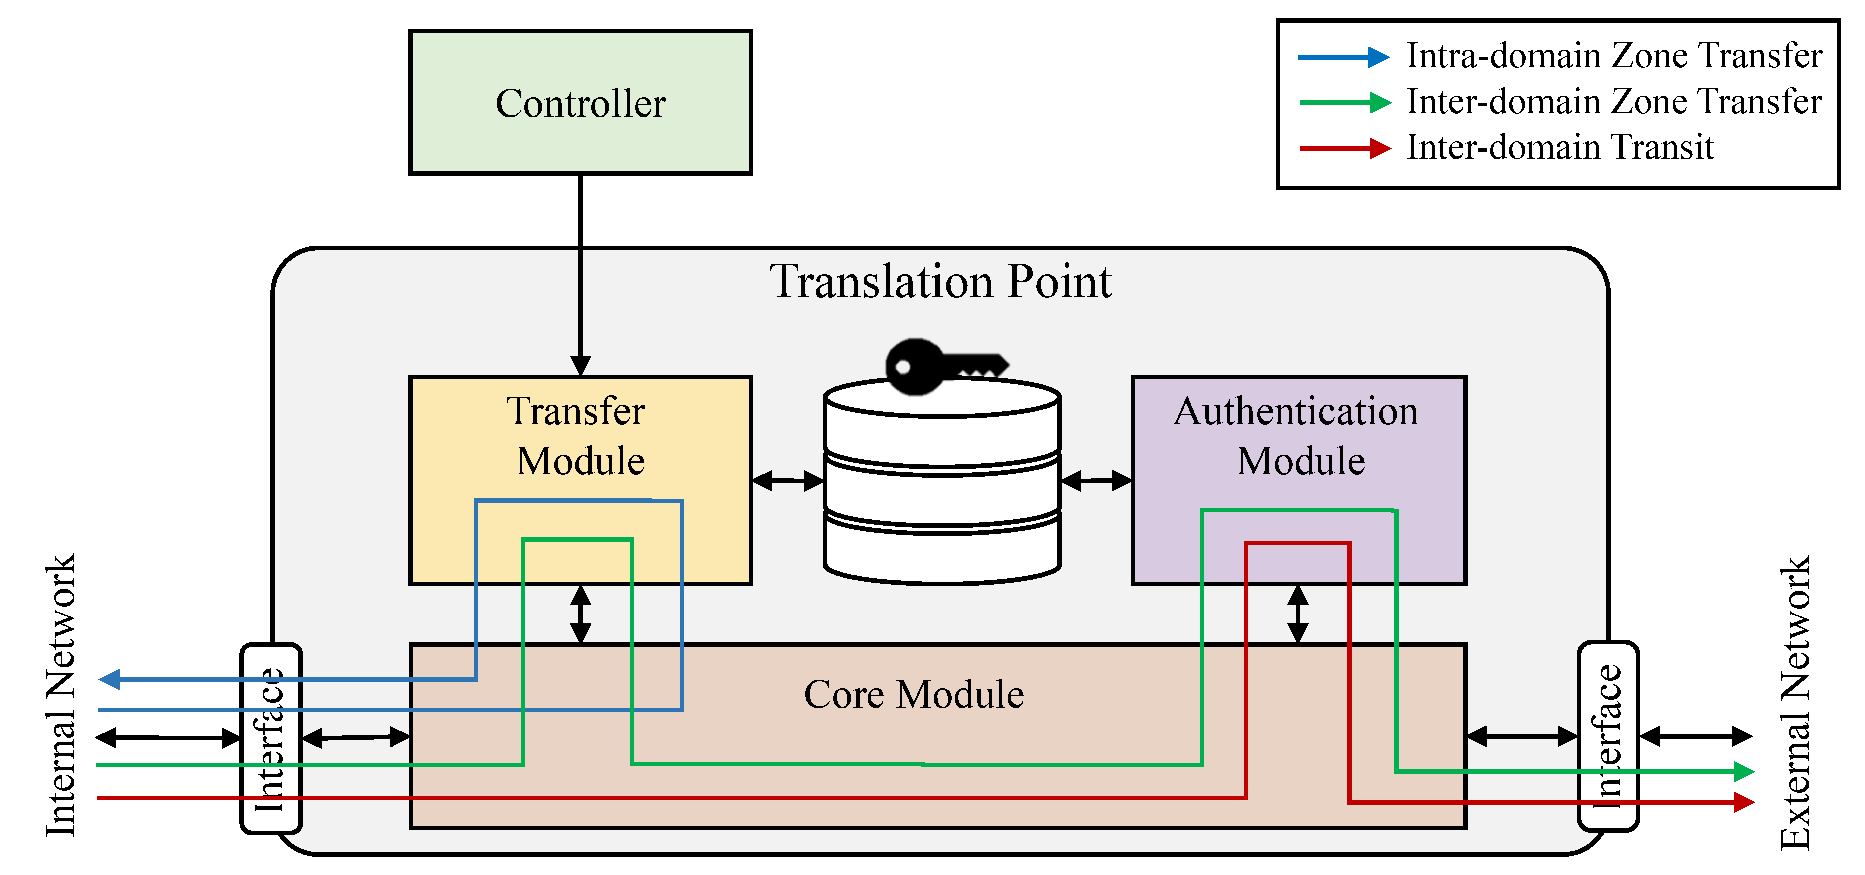
\includegraphics[width=0.9\textwidth]{tp.eps}
	\end{center}
	\caption{An overview of the modularized \tp implementation. Major usecases are also
		indicated with colored arrows.}
	\label{fig:tp}
\end{figure}

To implement a prototype of \tp, we extend the \fnurl{SCION-IP Gateway (SIG)}{https://github.com/scionproto/scion}.
The main functionality of SIG is to encapsulate legacy IP packets into SCION packets and
vice versa. In this context, a SIG acts as a gateway between an internal (legacy) network
and an external (SCION) network. Since \tp is designed as a gateway that bridges LAN
traffic over WAN---the underlying inter-domain routing protocol is not relevant here---the
functional aspects of \tp meets with what SIG provides. To be integrated with SIG, \tp
mediates between the UNIX socket and SIG socket, and performs zone transfer authorization
and verification for all incoming/outgoing packets.
Figure~\ref{fig:tp} illustrates
the implementation details of the modularized \tp design that consists of three main modules: i) core module, ii) transfer module, and iii) authentication module.
Here we describe the three main modules of \tp: i) core module, ii) transfer module, and iii) authentication module.

\paragraph{Core Module}
The core module is the main loop of \tp. It reads packets from the UNIX socket and
redistributes them to the corresponding interfaces. More precisely, when receiving packets
from the internal network, it retrieves metadata (further illustrated in
Appendix~\ref{apdx:meta}) from the raw packet, and hands over to the transfer module.
If the zone transfer is authorized ($return=1$),
the packet is then either forwarded back to the internal network or, in case the given destination is in a remote zone, once again handed over to the authentication module to be prepared for secure transmission.
For packets coming from the external network, \tp first calls the authentication module for
verification of the conveyed authentication token. Packets with invalid tokens are simply discarded.

\paragraph{Transfer Module}
The main objective of this module is to check the zone transfer rules. The transfer
module communicates with its controller to maintain a list of up-to-date zone transfer policies.
To this end, it establishes a TLS channel with the controller, downloads policies,
and populates the database.
We implemented the transfer module to support different drop-in options using APIs.

\begin{itemize}
	\item No-Op: This is for a setup in which no inter-domain zone transfers are required,
	      but only inter-domain zone extensions.
	\item Standard: This mode would perform an authorization check for the requested
	      zone transfer based on the source and destination IP addresses.
	\item Firewall: If needed, the module could be instantiated as a full-fledged firewall.
	      This mode would be useful for cases where the firewall can not be replaced.
	      \cmnt{should we discuss this further in the discussion section?}
\end{itemize}

\paragraph{Authentication Module}
For inter-domain packet transmissions, the authentication module issues an
authentication token for the packet. It (ideally) caches the first-level keys prefetched
from other \tps and derive a second-level key to generate the authentication token.
Inversely, for packets from other \tps, it derives the corresponding 2nd-level key
and verifies the delivered authentication token. \cmnt{explain implementation in more detail}

\begin{lstlisting}[
	basicstyle=\footnotesize, language=golang,
	caption={\textit{The KeyManager interface used to by the authentication module to fetch and
	derive keys.}},
]
// KeyManager is a thread-safe key store managing L0 and L1 keys
type KeyManager interface {
	// FetchL1Key fetches the level 1 key to be used to send
	// data to remote. It returns the key and a bool
	// indicating if the cached key was expired and a fresh
	// key has been fetched from remote.
	FetchL1Key(remote string) ([]byte, bool, error)
	// FetchL2Key fetches the Level-2 key used to encrypt
	// outgoing traffic
	FetchL2Key(remote string, zone uint32) ([]byte, bool, error)
	// Derive L1Key derives the level 1 key used to derive
	// the L2 key.
	DeriveL1Key(remote string) ([]byte, error)
	// Derive L2Key derives the level 2 key used to verify
	// incoming traffic.
	DeriveL2Key(remote string, zone uint32) ([]byte, error)
}
\end{lstlisting}

\paragraph{Database}
The \tp's database consists of three tables: \textit{Zone Table}, \textit{Zone Transfer
	Table}, and \textit{Key Table}. The zone table is used to map hosts to their corresponding
zones. For a fast table lookup, we leverage Radix Trees (also known as a trie or compact prefix
tree), \fnurl{cidranger}{https://github.com/yl2chen/cidranger} in particular. The zone transfer table is a database
in which the zone transfer rules are stored. The two tables are populated with the information
acquired from the controller. The key table is where the shared first-level keys are
accumulated.

\section{Controller}
\label{sec:controller}

We implemented the controller as a Web server written in golang with an SQLite database storing the
zone information and transfer policies. The controller offers an API which allows
\tps to fetch zoning information via HTTPS GET requests.

\paragraph{APIs}
The endpoints of interest are:
\begin{enumerate}
    \item \code{/api/get-subnets}
    \item \code{/api/get-transfers}
\end{enumerate}
Using these endpoints \tps fetch IP subnet and zone transfer rules. Important to note is that
the controller only hands out the subset of the full set of rules which is required for the
requesting \tp to be operational. This minimizes the size of data transmissions and also
improves security by not disclosing the full network view to every \tp. For every call to the
API the controller first verifies the authenticity of the caller before the request is forwarded
to the corresponding handler. The handlers then load the requested data from the database and
send it to the caller as JSON-formatted bytes.

\paragraph{Database}
The database consists of four tables (Zones, Sites, Subnets, Transfers), each describing one of
the core elements of the architecture.
The database schema is listed in the Appendix~\ref{apdx:controllerdb}. An abstraction layer
written in golang allows the controller to interface with the database using high-level calls.
The abstraction layer makes use of transactional queries to ensure consistency even in the event
of errors. Furthermore, the abstraction uses prepared statements for insertions, deletions and
retrievals of data. This protects against SQL-injections and improves the speed of queries.


\section{Authentication Token}
\label{sec:token}

\begin{figure}[htb]
	\begin{center}
		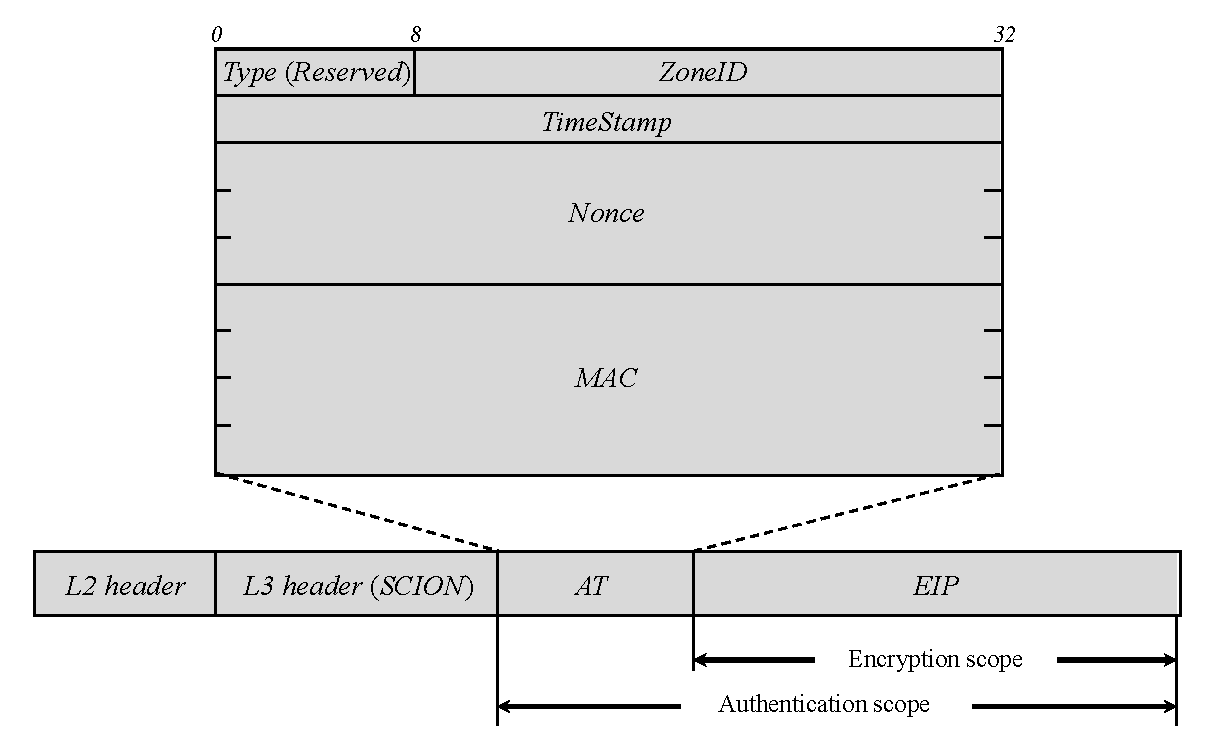
\includegraphics[width=.9\textwidth]{header.eps}
	\end{center}
	\caption{\name packet format for secure tunneling.}
	\label{fig:header}
\end{figure}

The \name packet format follows the IP tunneling conventions of encapsulating the original
packet with a new outer IP header that indicates the two tunnel endpoints as the new source
and destination. The original packet is encrypted and then authenticated along with the new
packet header fields. Figure~\ref{fig:header} shows the detailed packet structure and coverages
of the confidentiality and integrity guarantee.

The authentication token starts with one byte of reserved space for a \textit{Type} field. While
currently unused this will be useful in the future for distinguishing different variations of
the authentication token. \textit{ZoneID} depicts the 3 byte long zone identifier of the
destination zone. It is used by the receiving \tp to derive the correct key for MAC verification
and decryption. The next 4 bytes are occupied by a \textit{TimeStamp} which is added by the
sending \tp. It is the Unix time at the point of sending the packet. The receiving \tp uses this
timestamp to reject replayed packets. The timestamp is followed by a \textit{Nonce} of 12 bytes.

The nonce as well as the previous three token fields and the data to be encrypted (\textit{EIP})
serve as input to a \textit{Galois/Counter Mode} (GCM) algorithm with an underlying
\textit{AES-128} block cipher as cryptographic primitive. This mode of operation is widely
adopted for its performance as well as the capability to do \textit{authenticated encryption
	with associated data} (AEAD). Here it provides authenticity over the header fields
(\textit{Type}, \textit{ZoneID}, \textit{TimeStamp}) and the data in \textit{EIP} while
\textit{EIP} additionally also gets encrypted.

The 16 byte \textit{MAC} generated by GCM is the last field in the authentication token. Both,
the nonce and the MAC sizes follow the guidelines recommended by NIST SP 800-38D \cite{nistgcm}.

Listing~\ref{lst:transformer} shows the interface that is used by the authentication module
to create and attach an authentication token to an IP packet. Of particular interest are the
functions \code{ToIR} and \code{FromIR}. \code{ToIR} takes the raw
\code{packet}, a \code{key} and some metadata (\code{remote}, \code{dstZone}) and returns the
encrpyted packet with attached tag and an error. The error is \code{nil} if the
call was successful.
Inversely, \code{FromIR} receives an encrypted packet with attached token (\code{cipher}) and
a \code{key} and then returns the decrypted \code{packet} together with the token (\code{additionalData})
and an error. The error is again \code{nil} if the
call to the function was successful.

\begin{minipage}{\linewidth} % minipage makes the listing not split
	\begin{lstlisting}[
		basicstyle=\footnotesize, language=golang,
		label={lst:transformer},
		caption={\textit{The Transformer interface used by the authentication module 
		to create and verify authentication tokens.}},
	]
	// Transformer transforms IP packets to and from intermediate
	// representation
	type Transformer interface {
		// ToIR transforms packet to intermediate
		// representation.
		ToIR(remote string, key, packet []byte, dstZone uint32)
			([]byte, error)
		// FromIR transforms cipher from intermediate representation
		// back to a regular IP packet
		FromIR(key, cipher []byte)
			(additionalData []byte, packet []byte, err error)
		// ResetState resets the nonce state for remote	
		ResetState(remote string) error
		// GetZone retrieves the zoneID encoded in token
		GetZone(token []byte) (uint32, error)
	}
	\end{lstlisting}
\end{minipage}
 % Updated components / New components
\chapter{Evaluation}
\label{eval}

% With the prototype implementation, we conduct extensive evaluation including 
% system/network-wide benchmarks. 

\section{System Benchmarks}
\label{sec:systembenchmark}

% \paragraph{Experimental Setup}
We first conduct microbenchmark tests to evaluate the performance of \tp including the key
derivation, packet authentication, and authorization. For scrutinize and reproducible evaluation,
we leverage the standard benchmark library \texttt{testing} officially supported by golang.
The benchmarks are conducted on commodity machines equipped with an Intel i7 \SI{2.9}{GHz}
CPU, \SI{16}{GB} memory, and a \SI{1}{GbE} NIC.

\begin{table}[htb]
	\begin{minipage}{.47\linewidth}
		\caption{Benchmark results for the transfer policy lookup (ns).}
		\label{tab:authorization}
		\begin{tabularx}{1\linewidth}{X|XXXX}
			\toprule
			\# of Policies & No Miss & Src IP Miss & Dest IP Miss & Policy Miss \\
			\midrule
			100            & 312     & 100         & 235          & 313         \\
			\SI{1}{K}      & 399     & 105         & 264          & 394         \\
			\SI{10}{K}     & 381     & 99          & 262          & 386         \\
			\SI{100}{K}    & 448     & 101         & 290          & 435         \\
			\bottomrule
		\end{tabularx}
	\end{minipage}\hspace{2em}
	\begin{minipage}{.47\linewidth}
		\caption{Sender-side L1 key lookup and L2 key derivation times for different network sizes (ns).}
		\label{tab:derivation_send}
		\begin{tabularx}{1\linewidth}{X|XX}
			\toprule
			\# of Branches & 1st-level Key & 2nd-level Key \\
			\midrule
			100            & 154           & 88            \\	% 618-530=88
			\SI{1}{K}      & 155           & 97            \\	% 627-530=97
			\SI{10}{K}     & 161           & 175           \\	% 705-530=175
			\SI{100}{K}    & 157           & 111           \\	% 641-530=111
			\bottomrule
		\end{tabularx}
	\end{minipage}\vspace{2em}
	\begin{minipage}{.47\linewidth}
		\caption{Receiver-side L1/L2 key derivation times for different network sizes (ns).}
		\label{tab:derivation_rec}
		\begin{tabularx}{1\linewidth}{X|XX}
			\toprule
			\# of Branches & 1st-level Key & 2nd-level Key \\
			\midrule
			100            & 188           & 104           \\	% 508-404=104
			\SI{1}{K}      & 188           & 104           \\	% 508-404=104
			\SI{10}{K}     & 197           & 103           \\	% 507-404=103
			\SI{100}{K}    & 188           & 104           \\	% 508-404=104
			\bottomrule
		\end{tabularx}
	\end{minipage}\hspace{2em}
	\begin{minipage}{.47\linewidth}
		\caption{Processing times for the encryption/decryption for different packet sizes (ns).}
		\label{tab:authentication}
		\begin{tabularx}{1\linewidth}{X|XX}
			\toprule
			Packet Size (byte) & Encryption & Decryption \\
			\midrule
			100                & 856        & 659        \\
			500                & 1082       & 747        \\
			1000               & 1338       & 850        \\
			1500               & 1557       & 950        \\
			\bottomrule
		\end{tabularx}
	\end{minipage}
\end{table}

\paragraph{Authorization}
% The \tp's transfer module performs zone transfer authorization for every incoming packets.
\cmnt{adapt text to reflect new table}
From a technical perspective, the zone transfer authorization consists of two tree searches followed
by a database lookup;
upon receiving the packet metadata from the core module, the transfer module first looks
up the corresponding zone identifiers for the source and destination addresses, and then
compares them to the zone transfer policies. The authorization performance is therefore
dependent on the lookup time of the trees and the policy database.

Table~\ref{tab:authorization} shows
the benchmark results of database lookups for different numbers of policies.
Note that each benchmark ran a couple million iterations and kept the mean value.
The authorization check takes approximately 300 to \SI{500}{ns} per packet, which is a
notable result considering: i) a single lookup consists of two tree searches and a database lookup, ii) the result
is from a high-level language implementation, and iii) the test set scales 1000 times.
As expected, a lookup failure is commonly 24 to 31~\% faster than a successful lookup.
This implies that abnormal packets with invalid zone transfer requests can be quickly
discarded.


\paragraph{Key Derivation}
% When a \tp handles an inter-domain zone transfer packet, the \tp need to derive a correct 
% key for the authentication. As we described in~\S\ref{ssec:keymanagement}, the key derivation
% comprise with two steps: fetch the first-level key from the cache, and dynamically derive the 
% second-level key from the first-level key. 
% To securely forward a zone transfer packet over the public Internet, a \tp first 
We investigate the key derivation performance. Recall that the key derivation proceeds
differently for sender and receiver. A receiver is capable of directly deriving the
second-level key from the local secret (Eq.~\ref{eq:1stkey} \& Eq.~\ref{eq:2ndkey}),
whereas a sender needs to fetch the first-level key from the key cache before it can derive the second-level key.
From a scalability perspective, we vary the number of branches (a \tp for each) by increasing the number of stored
first-level keys up to \SI{100}{K}. Table~\ref{tab:derivation_send} depicts the average time for sender-side key derivation
measured by a benchmark running more than a million iterations. Table~\ref{tab:derivation_rec} shows the same results for
receiver-side key derivation. As can be seen, looking up the first-level key from cache is slightly faster than
deriving the first-level key from the local secret. This is expected when using a high-level language like golang.
Much faster key derivations are possible when using a state-of-the-art implementation \cite{rot2020piskes}.
On the other hand, the second-level key derivation takes roughly the same amount of time for sender- and receiver-side.
This is to be exptected as this derivation step is identical in both cases.

We observe that the lookup time for the first-level key is independent of the size of the key
table, taking between \SI{154}{ns} and \SI{161}{ns}. In addition, the size of the key table is
also irrelevant for the second-level key derivation
because second-level keys are directly derived from first-level keys.
The results indicate that the processing time for a key derivation is less than 1 $\mu$s
even in very large networks with \SI{100}{K} branch sites, which is negligible considering
network latency in today's Internet.

\paragraph{Authentication}
The additional processing time for packet encryption and decryption is shown in
Table~\ref{tab:authentication}. In summary, it requires approximately 1.5 to 2.5 $\mu$s to
authenticate various sizes of packets. We note that the processing overhead occurs for the majority
of tunneling technologies that provide confidentiality for data transmission. The processing
time can be minimized with implementations using the Data Plane Development Kit
(DPDK)~\cite{dpdk} or by leveraging hardware dedicated to cryptographic
operations.

\section{Network Benchmarks}
\label{sec:networkbenchmark}

\begin{figure}[htb]
	\begin{minipage}{.47\linewidth}
		\centering
		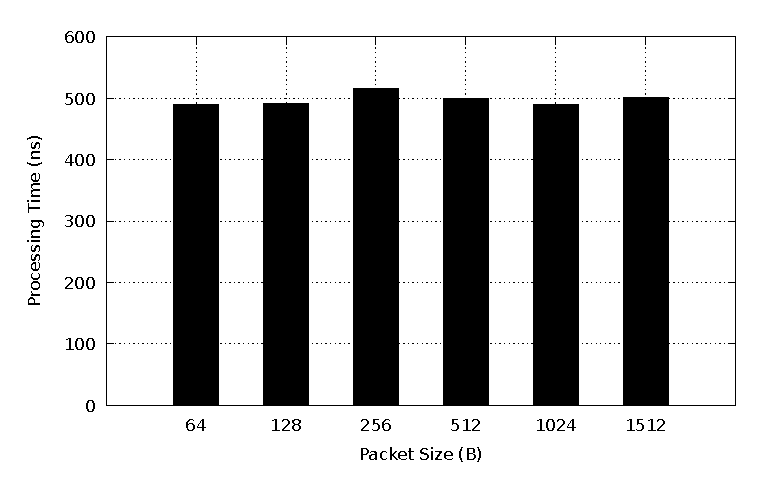
\includegraphics[width=\linewidth]{intra.eps}
		\caption{Processing time for intra-domain zone transfer.}
		\label{fig:intra}
	\end{minipage}\hspace{1em}
	\begin{minipage}{.47\linewidth}
		\centering
		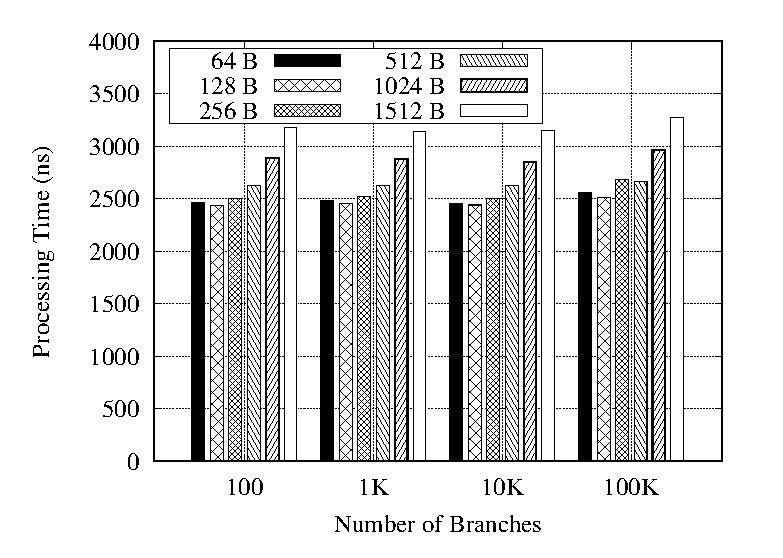
\includegraphics[width=\linewidth]{inter_sender.eps}
		\caption{Processing time on $TP_S$ for inter-domain zone transfer.}
		\label{fig:inter_sender}
	\end{minipage}\vspace{2em}
	\begin{minipage}{.47\linewidth}
		\centering
		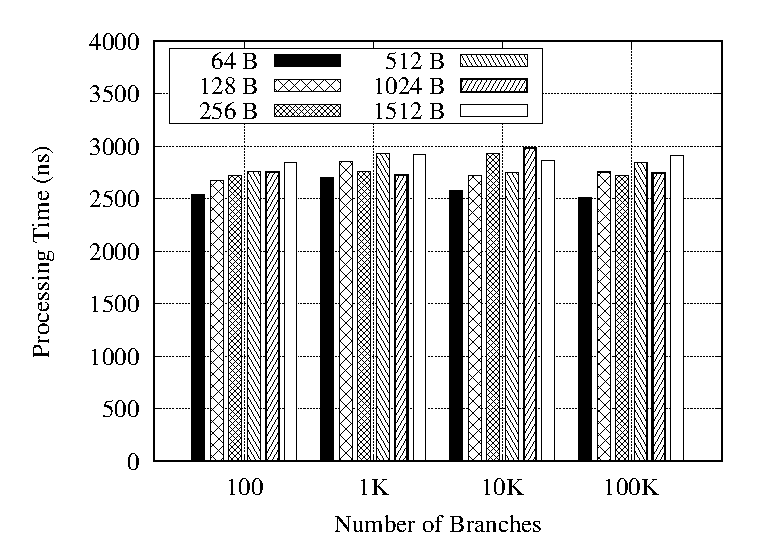
\includegraphics[width=\linewidth]{inter_receiver.eps}
		\caption{Processing time on $TP_R$ for inter-domain zone transfer.}
		\label{fig:inter_receiver}
	\end{minipage}\hspace{1em}
	\begin{minipage}{.47\linewidth}
		\centering
		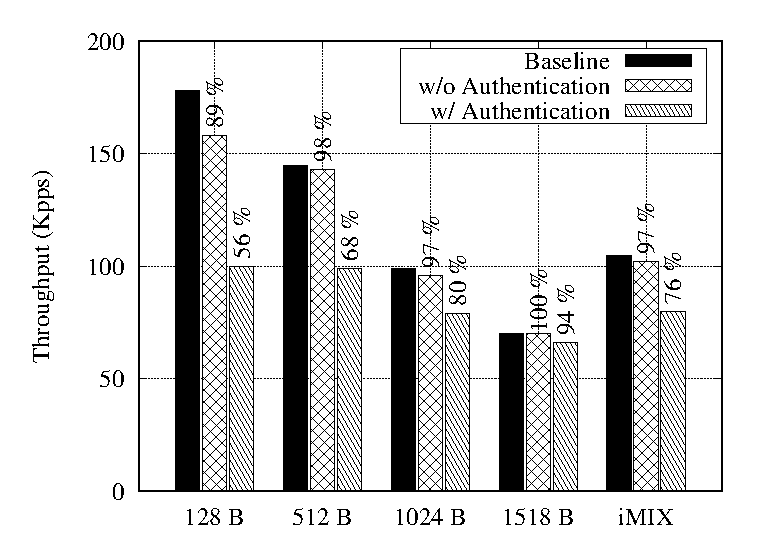
\includegraphics[width=\linewidth]{pps.eps}
		\caption{Forwarding performance of \tp for various size of packets.}
		\label{fig:forwarding}
	\end{minipage}\vspace{2em}
	\begin{minipage}{.47\linewidth}
		\centering
		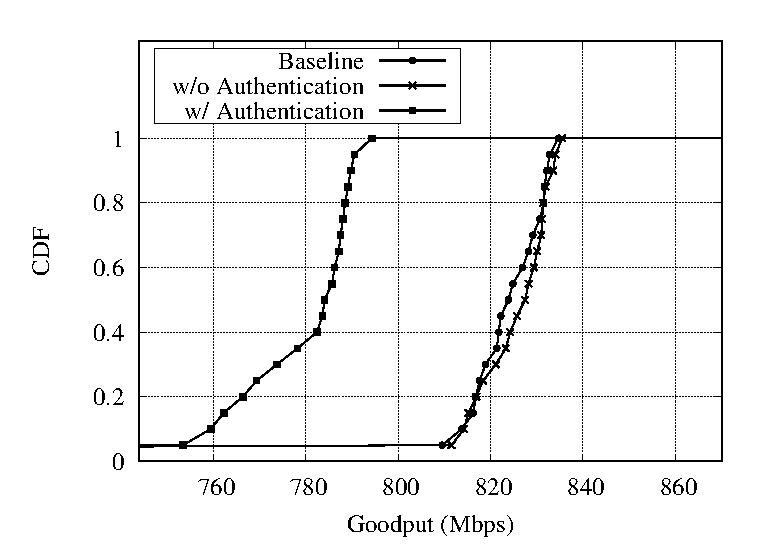
\includegraphics[width=\linewidth]{cdf_goodput.eps}
		\caption{CDF of goodput for 1400-bytes of maximum segment size (MMS).}
		\label{fig:goodput}
	\end{minipage}\hspace{1em}
	\begin{minipage}{.47\linewidth}
		\centering
		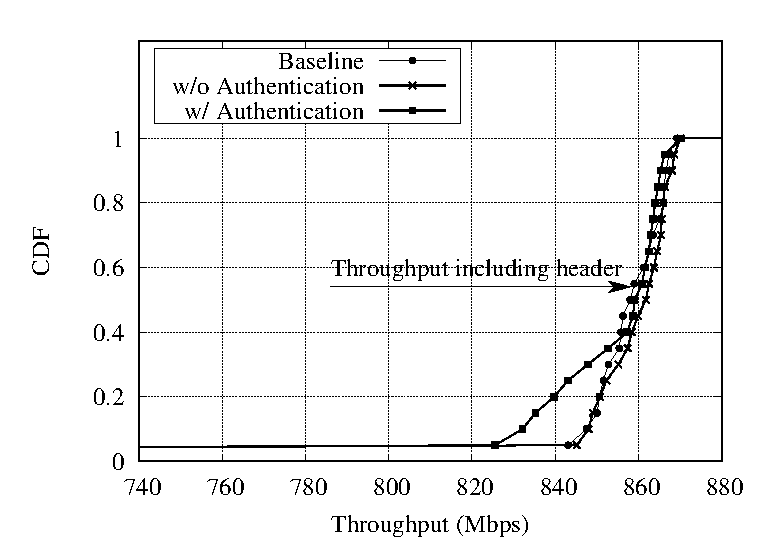
\includegraphics[width=\linewidth]{cdf_throughput.eps}
		\caption{CDF of throughput including extra header fields.}
		\label{fig:throughput}
	\end{minipage}
\end{figure}

So far, we evaluated the performance of each instruction newly introduced. Since a different
set of instructions needs to be applied depending on the zone transfer use case, it is also
important to investigate the overall network performance for handling different types of zone
transfer packets. We now benchmark the actual network performance for both intra- and inter-domain
zone transfer cases.

\paragraph{Latency Inflation}
Figure~\ref{fig:intra} illustrates the network benchmark results for the intra-domain zone
transfer where the source and destination zones are within the same local network, such that
the \tp only performs zone transfer authorization. Since no cryptographic operations are involved,
the additional latency is negligible (as a single legitimate zone transfer takes $\sim$
\SI{500}{ns}). There might be an authorization abort due to a lookup failure that could be
caused by the following three reasons: no matching source zone ID, destination zone ID, or
zone transfer policy. In our prototype, the lookups are performed sequentially and thus
there are different processing overheads (\SI{100}{ns} $\sim$ \SI{450}{ns}) depending on when a
lookup failure occurs. Nevertheless, in case there exists no valid zone-transfer policy, the
packet will be simply dropped and therefore no additional latency is caused.

For inter-domain zone transfer cases, we benchmark the overall network inflation during \tp
operations including packet parsing, key derivation, authorization, and authentication.
Figure~\ref{fig:inter_sender} and~\ref{fig:inter_receiver} depict the processing delay from
sender-side \tp and receiver-side \tp, respectively.
From the results, we make the following observations: first, the overall latency inflation that
\name introduces is insignificant ($\sim 3 \mu$s). Second, \name scales well with the size of the
network, i.e., the number of branches. We do not see any notable performance degradation
($\leq$ \SI{200}{ns}). Third, the size of a packet is the primary factor for the latency increment
as expected for all data-plane devices. The packet size has a small latency incremental factor of
1.28 (i.e, 2.4 $\mu$s to 3.8 $\mu$s). Lastly, we observe no significant bias in network
performance between sender-side and receiver-side \tps.


\paragraph{Forwarding Performance}
We further investigate the actual forwarding performance for various packet sizes (\SI{128}{B},
\SI{256}{B}, \SI{512}{B}, \SI{1024}{B}) including a representative mixture of Internet traffic
(iMIX)~\cite{rfc6985}; we select the minimum packet size of 128 bytes instead of 64 bytes which is
commonly considered to be the smallest packet size, because \name's tunneling requires an at least 116
bytes long frame, i.e., Outer L3 header (40 bytes), AT header
(36 bytes), and EIP (40 bytes). Figure~\ref{fig:forwarding} shows the results. The
baseline is the forwarding performance without \tp operations. The other bars represent the
forwarding performance for intra-domain zone transfer (with authorization only) and inter-domain
zone transfer (with authorization and authentication) respectively.

For 128-byte packets which demonstrates the highest packet rate, and thus requiring the most
extreme packet processing, the intra-domain zone transfer exhibits a throughput degradation
of only 11\%. For other packet sizes we achieve a throughput of 97 $\sim$ 100\%. These
results are expected because \tps only perform zone authorization for intra-domain zone transfer
packets, which increases processing delay by $\leq$ 500 ns. Considering that
a typical intra-domain packet transmission usually shows a few milliseconds of latency, the
additional delay is negligible.

On the other hand, the inter-domain zone transfer degrades the throughput by 44\% for the
smallest packets. Although the degradation diminishes as the packet size increases, the
performance still degrades by 24\% for the iMIX traffic. To investigate the main degradation
factor, we compare the amount of transmitted data (goodput) and the total bits transmitted
including all the network headers (throughputs) as shown in Figure~\ref{fig:goodput} and
\ref{fig:throughput}. From the comparison, we observe the followings: i) the inter-domain
zone transfer achieves a similar throughput to the baseline if the extra headers are considered,
ii) the performance degradation is caused by not only the additional processing delay but also
transmission delay of the extra headers, and therefore iii) \name performs similar to
today's tunneling applications while providing security policy enforcement for network
zoning.



% \subsection{Overhead Measurements}
% \label{ssec:overhead}

% \paragraph{Bandwidth Overhead}

% \paragraph{Memory Overhead}

% \paragraph{Control-plan Overhead}

 % Evaluation
\chapter{Security Analysis}
\label{analysis}

% Security analysis goes here.

% Compromise attack: sepration of key management from controller limites impact of 
% compromised controller. 

% Source spoofing from internal host -> internal network is assumed to be trusted.
% -> internal attacker does not know which IP address (or subnet) is allowed to
% access a target zone.
% -> port-based ingress filtering (enterprise network benefits from the deployment)

% We analyze the security properties that \name provides, considering the threat model
% introduced in \S\ref{ssec:threatmodel}. The attack classes described here are threefold:
% i) attacks to identify a target network structure in terms of security policies and their
% corresponding access hierarchies, ii) attacks to infiltrate restricted and highly secure
% zones without a proper permission, and iii) disruption attacks that destroy network 
% functionalities. For each attack class, we describe potential attack methodologies and
% mitigations.
We analyze the security properties that \name provides, considering the threat model
introduced in \S\ref{sec:threatmodel}. The attack classes described here are twofold:
i) attacks to infiltrate restricted and highly secure zones without a proper permission,
and ii) disruption attacks that prevent availability.
% For each attack class, we describe potential attack methodologies and mitigations.

% \subsection{Zone Structure Surveillance}
% \label{ssec:scanning}

% % In this attack class, we consider attackers sniffing the victim network to disclose
% % security vulnerabilities. Attackers often take a long breath to successfully breach 
% % the highly secure systems. By either passive monitoring or active scanning,
% % attackers attempt to draw a map of the target network and identify the topological
% % characteristics along the access controls. Note that, since this attack class is 
% % usually in preparation for major security breaches, we only consider attackers from 
% % offshore network.

% % \paragraph{Passive Monitoring}
% % Attackers may observe packets at the traffic aggregation points, e.g., routers and switches
% % at core networks. Since there are countless packet-sniffing tools and wire-tapping devices 
% % available in the market, indeed monitoring live traffic associated with the target network
% % is an effortless---just time consuming---and effective attack method; the header fields is 
% % already informative to the attackers because they expose the pairs of communicating hosts, 
% % enabling attackers correlating the hosts and their trust hierarchy. 

% In this attack class, we consider attackers sniffing the victim network to disclose
% security vulnerabilities. Note that, since this attack class is usually in preparation 
% for major security breaches, we only consider attackers from offshore networks.

% \paragraph{Passive Monitoring}
% Attackers often take a long breath to successfully breach the highly secure systems.
% Monitoring live packets at the traffic aggregation points (e.g., router and switches at the 
% core network) is definitely time consuming, but indeed an effective and effortless attack
% method; the packet header is already informative for attackers, as it exposes the pairs
% of communicating hosts, enabling attackers to correlate the observed hosts and their access
% hierarchy (i.e., zone map). In addition, there are countless packet-sniffing tools and 
% wire-tapping devices available on the market. 

% Nonetheless, \name's secure tunneling for the inter-domain zone transfer prevents passive 
% monitoring from sketching the zone map. It only exposes the IP addresses of the two tunnel endpoints,
% while keeping data confidentiality and communication privacy by encrypting the original IP 
% packets. Although a \name packet conveys the destination zone ID in the AT header field, it
% only depicts what zones are under the destination \tp. Furthermore, the zone ID is an
% arbitrary number, and therefore it is impossible to infer the underlying security policies.

% \paragraph{Active Scanning}
% Attackers may perform active scanning to identify a vulnerable spot by transmitting forged
% packets to a specific host residing in a trusted zone. To this end, the attackers however
% must pass through the authentication check which requires a correct cryptographic key.
% Since the key binds to the triplet of \{$\tp_{src} | \tp_{dst} | zoneID_{dst}$\} and only
% the corresponding \tps can derive the correct key, scanning the network from outside
% is hardly possible. 


\section{Infiltration without a Permission}
\label{sec:infiltration}

Apparently, one of the main attack objectives is to access valuable information assets
protected by access constraints.

\paragraph{Man-In-The-Middle Attack}
To become ``in the middle'', an attacker could initiate independent communication channels
with two \tps and relay messages between them. By using the attacker's public key for the
channel establishments, the attacker is able to generate valid packets that can bypass the
\tp's authentication check.

\name's PKI design prevents the MITM attacks. A MITM attack
can succeed only if the attacker convinces each \tp that they are talking to each other.
In the process of secure channel establishment, however, \tps authenticate each other using
the certificates issued by the mutually trusted CA (e.g., enterprise). Since the attacker's
public key cannot be certified by a valid certificate issued by the CA, a MITM will fail.


\paragraph{Packet Replay}
Attackers can observe valid \name packets and then reuse them to transmit attack traffic.
Nevertheless, the validity of the reused packet header will be compromised once the payload
is changed---recall that the authentication scope covers the entire packet including
AT and EIP as shown in Figure~\ref{fig:header}---and therefore attackers cannot
successfully pass the authentication check at the recipient \tp.


\paragraph{Brute-force Attack}
Another approach is to brute-force the key used for authentication or the MAC. As we are using 128-bit cryptographic keys and MACs, such attacks are currently infeasible. To achieve resilience to quantum computers, the key size would need to be doubled, however.

% Attackers may
% generate all possible combinations to derive the valid key. To break the 128-bit symmetric
% key which has $2^{128} \approx {3.4e38}$ combinations, it requires $2.59e13$ years on the
% world's fastest supercomputer, Fugaku ($415.53e15$ Flops)~\cite{top2020supercomputer}, even 
% if we consider that a combination check requires just a single Flop.

% To brute-force the 128-bit MAC instead, it requires ${3.4e38}$ probes to be 
% transmitted, taking $6.38e22$ years on a {100} {Gbps} network link by using the smallest
% frame size of 74 bytes (i.e., Ethernet(18 bytes) + IP(20 bytes) + AT(36 bytes)).

\section{Denial-of-Service Attack}
\label{sec:disrupting}

\paragraph{Exhaustion Attack}
Flooding the \tp's authentication process could be an effective attack vector. Attackers
may attempt to forward a large number of packets to the target \tp in order to exhaust the
\tp's resources. Even if the attack packets contain invalid authentication tokens, the \tp still
needs to verify these tokens, therefore wasting resources, preventing legitimate packets from getting through.

To be resilient to such attacks, we consider operating multiple \tps at the entrypoints
of cooperative networks. Multiple \tps enables network operators
to load balance and easily switch over to another \tp in case of a link (or a \tp)
failure. In fact, many data centers and large enterprise networks already employ equal-cost
multipathing (ECMP)~\cite{rfc2991,rfc2992} along with multiple gateways and ToRs (Top-of-Rack
switches) to provide reliable intra-networking services. In addition, to mitigate possible DoS
attacks from the public Internet, Microsoft implemented a global ECMP
infrastructure~\cite{ms2020ecmp}. Path-aware networking along with multipath communication
% is also in the spotlights of both, industry and academia recently
also enables active switching to different entry points, if some fail or are under DDoS attack.~\cite{Dawkins2018,Trammell2018}.


% \paragraph{Fake \name entities}
% Another possible attack factor is to initialize a face \name entity. 
 % Security analysis
\chapter{Practical Considerations}
\label{practical}

In this chapter, we discuss some practical considerations including functional and
management aspects, along with various deployment scenarios describing how \name can
be realized on today's enterprise infrastructure.


\section{NAT Devices}
\label{sec:nat}
Multiple hosts connected through a NAT device appear as a single host to the
\tp. \textit{Internal} NAT devices hardly pose a problem since the hosts under that NAT
device are all subject to the same subnet and therefore belong to a single network zone.
Network operators establish a security policy on the translated IP address, such
that \tps are able to authenticate the zone transit requests from/to a host under the
internal NAT device.

However, an \textit{external} NAT device located in an external network, e.g., carrier grade NAT,
could affect the \tp's secure tunneling ability. The translated \tp's IP address
would cause a MAC verification failure---recall that each symmetric key binds to the
triplet including \tps' IP addresses as described in \S\ref{sec:keymanagement}.
This, however, can be addressed by enforcing \tps to use their public IP addresses
to derive the symmetric keys. The keys are still secure since the first-level key
from which the pairwise keys are derived is exchanged with the CA-certified public
keys. Discovering the translated \tp address is also not a problem thanks to
the controller informing senders about the recipient \tp's address (see Protocol 3 in
Figure~\ref{fig:protocol}).

A potential operational failure occurs where multiple \tps reside behind the same NAT
device. This would lead to remote \tps deriving identical keys for all the \tps
behind the NAT. One possible solution would be to use a unique \tp identifier
instead. Since all such \tps would be under one administration domain, assigning
unique \tp identifiers upon bootstrapping is feasible. Then, the \tps convey
their identifiers in the AT header field alongside the destination zone ID. This
might slightly increase the size of the header, but does not degrade the
security of the underlying authentication.


\section{Tunneling Granularity} %\paragraph{Zone-to-Zone VPN}
\label{sec:granularity}
% Thanks to the flexible and scalable key derivation scheme introduced in~\cite{rot2020piskes},
% the key establishment supports the secure tunneling in different granularities: 
% i) site-to-site tunneling, ii) zone-to-zone tunneling, and iii) site-to-zone tunneling 
% (the one we take). 
Secure tunneling can be realized in different granularities: i) site-to-site tunneling,
ii) zone-to-zone tunneling, and iii) site-to-zone tunneling (the one used by \name).

% Similar to IPSec VPN, the site-to-site tunneling requires a single symmetric key per
% a \tp pair, e.g., the first-level key. Indeed, the site-to-site key establishment is 
% already enough in terms of communication security and privacy for two tunnel endpoints. 
% However, this approach requires another step of zone transfer verification.
Similar to IPSec VPN, site-to-site tunneling provides strong guarantees about
communication security and privacy for two tunnel endpoints. However, from a
flexibility and manageability standpoint, having a site-to-site tunneling
architecture is not ideal. Every tunnel endpoint needs to share a key with every
other endpoint with which it wishes to exchange data. This adds state to the
endpoints that needs to be kept in sync. Adding a new site requires an update on
all the other sites that wish to communicate with the new site. Then, yet
another layer of security middleboxes (e.g., firewalls) are required to perform
zone transfer authentication since keys do not designate a specific zone.

An alternative way of providing authentication is to use one key per zone pair.
In this model, when a zone transfer is required, a \tp would sign the data on
behalf of the zones with the corresponding source/destination zone key pair.
This approach has the benefit that sender and receiver get decoupled as in
principle any site that possesses the right keys can perform that zone transfer.
Adding a new site would be as easy as fetching the right keys for the desired
zone combinations. This process is independent of all the other sites. However,
a receiver \tp needs to be able to fetch the right keys from the cache, in order
to derive second-level keys, which means that the zone transfer information must
be visible in plain text. Thus, an attacker could potentially learn the zone
structure of the observed network. Also, having a separate key per zone pair
does not scale since the number of zones gets big very quickly for large
networks.

Driven by these considerations, we designed the new concept of site-to-zone
tunneling, which represents a middle ground combining the advantages of the two
approaches, the notion of secure tunneling and zone transfer authentication. The
symmetric keys are distinguishable depending on the destination zone, while at
the same time the zone-to-zone security policies are not being exposed. Thanks
to the flexible and scalable key derivation scheme introduced
in~\cite{rot2020piskes}, the key establishment does not expand state, while
still providing unique symmetric keys per zone. Furthermore, this scheme scales
linearly with the number of sites, not the number of zones, which ensures
scalability.

\section{Distributed Controllers}
\label{sec:distributedcontroller}
Driven by the scalability and reliability issues inherent to a single physical
controller, namely \textit{single-point-of-failure}, logically centralized
control-planes built on physically distributed instances find wide acceptance in
the current practice. The most common approaches realizing distributed
controllers can be broadly categorized into horizontal
distribution~\cite{berde2014onos,medved2014opendaylight} and hierarchical
distribution~\cite{hassas2012kandoo,yap2017taking}. Independent of which
distribution architecture is used, we discuss location, coordination, and
migration aspects of distributed controllers.

\paragraph{Location}
The notion of a logically centralized control-plane offers flexibility in
network design and management. A key design choice is placement of the
(distributed) controllers, which could impact to performance, reliability, and
management scalability of a given network. There is comprehensive research on
the controller placement problem considering practical issues from control
latency to reliability, from cost-optimization to load balancing, and so
on~\cite{das2019survey,zhang2017role,he2019toward}. Among those, we are mainly
interested in the latency performance indicator; that is the latency between a
controller and regional forwarding devices.

The best latency is achieved when each branch site has its own controller. By a
placement near local \tps, the controller minimizes the \tp-controller latency
for the zone transfer authorization protocol, allowing instant feedback for
packet forwarding---we note that inter-controller communication for global
coordination is commonly not latency sensitive. For the sake of control-plane
security, the controller resides in a highly restricted zone to which only the
local \tps and remote controllers have access. Although the per-site controller
offers the best performance regarding policy enforcement for the data-plane,
there might be a cost-efficiency problem for a large-scale network with
thousands of branches.

Alternatively, we consider a sparse distribution model, e.g., on edge-cloud
systems. Similar to today's cloud services, network operators running
geographically distributed data centers can instantiate multiple controllers at
the central point of regional branches. The control-plane latency overhead would
be higher compared to the dense deployment model---if the data center edges are
geographically diverse, the overhead could be minimized---but, in terms of
cost-optimization and management scalability, it could be a more viable
approach.

\paragraph{Coordination}
It is important to keep consistency in global coordination across the
distributed controllers. Indeed, inconsistency in security policy might grant
hosts with a low security clearance unauthorized access to highly restricted
zones, resulting in unexpected information leakage and eventually administration
failure. With this in mind, we consider a consensus algorithm with strong
consistency guarantees~\cite{panda2013cap,phemius2014disco,shi2014giraffe},
where the security policy is dynamically shared/replicated across the
distributed controller instances, ensuring concurrent policy enforcement towards
the data-plane devices. There are numerous open-source projects, such as
\fnurl{Consul}{https://github.com/hashicorp/consul}, \fnurl{Apache
	ZooKeeper}{https://zookeeper.apache.org/}, and
\fnurl{ETCD}{https://github.com/etcd-io/etcd} available.

\paragraph{\tp Migration}
To benefit from the distributed controller environment, a dynamic controller discovery
process also becomes important. That is, \tps should be able to search a cluster of best
candidates, diagnose the performances of control latency, and seamlessly migrate to the
best controller. To this end, we consider a two-step migration process: i) \tp-driven
control channel initialization and ii) controller-driven \tp migration.

\tps are responsible for establishing the first control plane channel with a controller.
For example, a new \tp ($\tp_{new}$) has been configured to contact an initial controller
acting as a first rendezvous point.
% \claude{a tp has been configured with an initial controller address acting as rendez-vous point?}
The initial information contains the controller's IP address
($C$), the corresponding zone ID ($Z_{C}$), and the \tp's IP address behind which the controller
resides ($\tp_{C}$). If the controller is located in a remote site (i.e., $\tp_{new}
	\neq \tp_{C}$), $\tp_{new}$ should connect with $C$ through $\tp_{C}$. Otherwise, e.g.,
$C$ is within the same LAN or in public network, $\tp_{new}$ can directly send $C$ a request
for control-plane channel establishment.

Once the \tp joined the network, the controller then initiates a migration process to
find the best controller ($C_{best}$) for $\tp_{new}$. Upon a migration request broadcasted
by $C$, other controllers measure the possible latency to $\tp_{new}$ and reply back
the results. Then, $C$ elects $C_{best}$ considering the latency measurements and the
current load balance, and sends $\tp_{new}$ a \texttt{RoleChange()} request containing
$C_{best}$, $Z_{C_{best}}$, and $\tp_{C_{best}}$. Finally, $\tp_{new}$ swaps the best
controller by establishing a new channel with $C_{best}$. The migration process
is also applied when changes in the network are detected.


\section{Nonce Reset}
\label{sec:nonce}

\begin{table}[htb]
	\footnotesize
	\caption{Comparsion of different nonce creation strategies. \texttt{l} is the length of the
		nonce, \texttt{s} $\leq$ \texttt{l} is the subset of bits reserved for the random part of the nonce,
		\texttt{p} is the number of nonces generated and \texttt{r} is the number of unplanned nonce
		resets.}
	\label{tab:nonce}
	\renewcommand\arraystretch{2}
	\begin{tabularx}{1.1\linewidth}{|X|X|X|X|X|X|}
		\hline
		                                        & \textbf{requires randomness}                       & \textbf{requires non-volatile memory} & \textbf{overlap probability w/o
		resets}                                 & \textbf{overlap probability for \texttt{r} resets} & \textbf{overlap}                                                                                                    \\
		\hline
		\textbf{counter only}                   & no                                                 & no                                    & 0                               & 1                                  & full \\
		\hline
		\textbf{randomness only}                & yes                                                & no                                    &
		$1-\frac{(2^l)!}{2^{l*p}(2^l-p)!}$
		                                        & $1-\frac{(2^l)!}{2^{l*p}(2^l-p)!}$                 & partial                                                                                                             \\
		\hline
		\textbf{counter paired with randomness} & yes                                                & no                                    & 0                               & $1-\frac{(2^s)!}{2^{s*r}(2^s-r)!}$
		                                        & full                                                                                                                                                                     \\
		\hline
		\textbf{reset points}                   & no                                                 & yes                                   & 0                               & 0                                  & -    \\
		\hline
	\end{tabularx}%
\end{table}

% Authenticators are created using an AEAD algorithm with an underlying AES-128 cipher in GCM mode.
% GCM requires a nonce as input argument to build counters which are then used to create the
% keystream. 
The same nonce must never be used twice with the same key, otherwise the security of the
cipher significantly decreases. In theory it is easy to create nonces that fulfill this
requirement. One can simply use a counter which is increased for every invocation of the
AEAD algorithm. In real systems this is not so easy to achieve since machines can crash
and lose their state, specifically their nonce counter. Outlined below are some techniques
to approach this problem.

\begin{itemize}
	\item \textit{Purely random nonce}: uses all bits of the nonce for randomness. Low
	      probability for overlap but no guarantee even when no resets.
	\item \textit{Counter paired with random sequence}: divides the nonce into a counter
	      and a randomized part. Initialize the random part after every restart and increase
	      the counter part for every packet. On reset start counter from zero with a fresh
	      randomized part. In case of overlap all packets do overlap.
	\item \textit{Reset points}: defines specific resets points for the counter which are
	      stored on non-volatile memory (NV-memory). Increment counter in memory and write the
	      next reset point to NV-memory when threshold is crossed. On crash restart counter from
	      reset point on NV-memory.
\end{itemize}

Table~\ref{tab:nonce} shows a comparison of the mentioned approaches. For this work, we chose the
approach of pairing an 8 byte counter with 4 bytes of randomness ($\texttt{s} = 32$) to obtain a 12
byte nonce. An example calculation shows that for $\texttt{r} = 10'000$ resets, the probability of
a nonce clash is still only $\sim$1.16\%.

\cmnt{uncomment DMZ section}
% \subsection{DMZ Traffic}
% So far, we mainly described on how two \tps can securely communicate each other. However,
% since most of cooperative information systems have public services facing the public Internet,
% we also need to consider 

% DMZ is a zone hosting public services. Since access traffic to the public services is 
% mostly originated from public Internet, 

\section{Fast Failover}
\label{sec:ecmp}
Operating multiple \tps with advanced ECMP-enabled layer 2 protocols (e.g., SPB and
TRILL) is a viable network design that provides load balancing and enhanced resiliency
against a \tp or link failure, as we discussed in \S\ref{sec:disrupting}.
If a \tp is unable to continue data transmission, ECMP engages. It searches an alternative
forwarding path considering cost equality and redirects flows through the new path, assuring
continuous communication for end hosts~\cite{rfc6754}.
This elastic migration during a transient network outage, however, does not replicate the
forwarding state of each flow, and thus might require another step of repopulating
forwarding state. Upon packet arrival, the new \tp fetches the zone transfer policy
and caches it in the forwarding table. Note that for \texttt{established} connections this might
cause unexpected packet drops if the first packet is a response. Nevertheless, the
communication would continue as soon as the original sender notices the packet drop
and requests a retransmission.

\cmnt{uncomment cross-enterprise section}
% \subsection{Cross-enterprise Setup}
% \label{ssec:crossconnection}
% Collaborators may join to an enterprise network. To be able to access highly secure zones
% in the enterprise network, the collaborators need to satisfy the following administrational
% and technical constraints: i) the collaborators must acquire a proper access grant from
% the enterprise's administration, and ii) install a \tp at their network.

% The enterprise network would have a single administration domain as we assumed
% in~\S\ref{ssec:assumptions}. To allow the collaborators interconnect their network system

% \subsection{\tp Deployment}
% \label{ssec:deployment}

% From a technical perspective, a \tp has obligations of: i) interconnecting VLANs , ii) 
% fetching security policies from the controller, and iii) enforcing the policies. 


% \paragraph{Gateway}
% A gateway 


% \paragraph{Middlebox}



\section{Incremental Deployability}
\label{sec:deployability}

To be incrementally deployable, \name does not require changes from end hosts nor the local network
infrastructure. \name can take a supportive role by complementing already installed lines of defense
such as firewalls, IPS, and IDS. For instance, traffic can be pre-filtered by \tps before it reaches
firewalls located deeper inside the network. This approach favors an incremental deployment
strategy. On the other hand, \name can also be used as a single, all-in-one solution providing
packet filtering, tunneling, and routing within one device. Such a deployment is especially
interesting for small branch sites with much simpler network layouts. Here, \name can drastically
reduce the number of devices that need to be maintained.



 % considerations for deployability
\chapter{Conclusion}
\label{concl}

\section{Summary}
\label{ssummary}

Network zoning has long been recognized as the cornerstone of secure network
operation and management. In the current practice, operators realize network
zones with network segmentation technologies and security middleboxes. As
information systems become more dynamic from a topological, operational, and
functional perspective, however, the conventional network-zoning architectures
face new challenges in terms of scalability and flexibility. In this thesis, we
have shown that lightweight policy enforcement for inter-zone communication is
achievable. Following a constructive approach with a cryptographic foundation,
it is possible to create a proactive alternative to the mostly reactive systems
presently used in network zoning. In conjunction with \name, verification based
on firewalls becomes simpler because firewalls would only process a limited
amount of (filtered) traffic. \name consequently reduces the number of
management points of distributed networks while retaining a high degree of
security.

\section{Future Work}
\label{sfuture}

The work presented in this thesis can be extended along different axes. For
one, it would be interesting to explore how an architecture like \name can be
used to provide privacy for inter-domain data transmissions. \name provides
confidentiality and integrity on the data in transit. However, certain traffic
patterns and packet sizes could still allow an attacker to draw conclusions about
what sort of traffic is being sent (\eg sensor data, control messages, file
transmissions) and which security zones are located
at a given site. If privacy is a concern, a first step could be to extend \tps
with new modules that pad all packets to the full MTU length and insert mock
traffic, such that traffic patterns are hidden.

Another direction in which this work could be extended is the implementation
of the \tp gateway in a high-performance language. Various operations---in
particular cryptographic ones---would benefit from an optimized
implementation on dedicated network hardware.

Lastly, it would be interesting to explore how certain properties of local
networks can be conveyed across the WAN to a remote network. For example, technologies such as
SPB and TRILL have support for layer 2 multipathing, the corresponding control
messages are, however, not transmitted by \name. A deeper interoperability of
different protocols across network boundaries would certainly be a desirable property.
 % Conclusion

\appendix

\chapter{Packet Metadata}
\label{apdx:meta}

%\section{Packet Metadata}
%\label{apdx:metadata}

\begin{lstlisting}[
	basicstyle=\footnotesize, language=golang,
]
type Packet struct {
	Ingress		bool
	SrcHost 	net.IP
	DstHost 	net.IP
	RemoteTP	string
	DstZone		uint32
	RawPacket 	common.RawBytes
}
\end{lstlisting}

The packet metadata is the abstract object passed between modules, describing an IP packet.
It accumulates information about the raw IP packet (\texttt{RawPacket}). The \texttt{Ingress}
field identifies a packet as either an ingress packet, coming from the WAN, or an egress packet
that originated in the local network. \texttt{SrcHost} and \texttt{DstHost} reflect the source
and destination IP addresses of the packet. \texttt{RemoteTP} designates the remote \tp. For an
ingress packet that is the source \tp from which the packet was received, for an egress packet
it is the \tp to which the packet needs to be forwarded to. \texttt{DstZone} is the Zone ID of
the zone to which \texttt{DstHost} belongs.

\chapter{Controller Database}
\label{apdx:controllerdb}


\begin{lstlisting}[language=sql, basicstyle=\tiny, %or \small or \footnotesize etc.
]
CREATE TABLE Zones(
id INTEGER NOT NULL,
name TEXT,
PRIMARY KEY(id)
);

CREATE TABLE Sites(
tp_address TEXT NOT NULL,
name TEXT,
PRIMARY KEY(tp_address)
);
	  
CREATE TABLE Subnets(
net_ip BLOB NOT NULL,
net_mask BLOB NOT NULL,
zone INTEGER NOT NULL,
tp_address TEXT NOT NULL,
PRIMARY KEY (net_ip, net_mask),
FOREIGN KEY (zone) REFERENCES Zones(id) ON DELETE CASCADE,
FOREIGN KEY (tp_address) REFERENCES Sites(tp_address) ON DELETE CASCADE
);
	  
CREATE TABLE Transfers(
src INTEGER NOT NULL,
dest INTEGER NOT NULL,
PRIMARY KEY (src, dest) ON CONFLICT REPLACE,
FOREIGN KEY (src) REFERENCES Zones(id) ON DELETE CASCADE,
FOREIGN KEY (dest) REFERENCES Zones(id) ON DELETE CASCADE	
)
\end{lstlisting}

The controller database consists of 4 tables: \texttt{Zones}, \texttt{Sites}, \texttt{Subnets},
and \texttt{Transfers}. The \texttt{Zones} table contains all network zones known to the
controller, identified by zone IDs. Additionally, a human readable description is attached. The
\texttt{Sites} table holds all known branch sites with the addresses of the corresponding \tps
and a textual description. The \texttt{Subnets} table describes the configured IP subnets
together with their zone membership and the \tp behind which they are located. Finally, the
\texttt{Transfers} table reflects the zone transfer matrix of allowed zone transfers.

\backmatter

\bibliography{refs,rfc}
\bibliographystyle{unsrtnat}

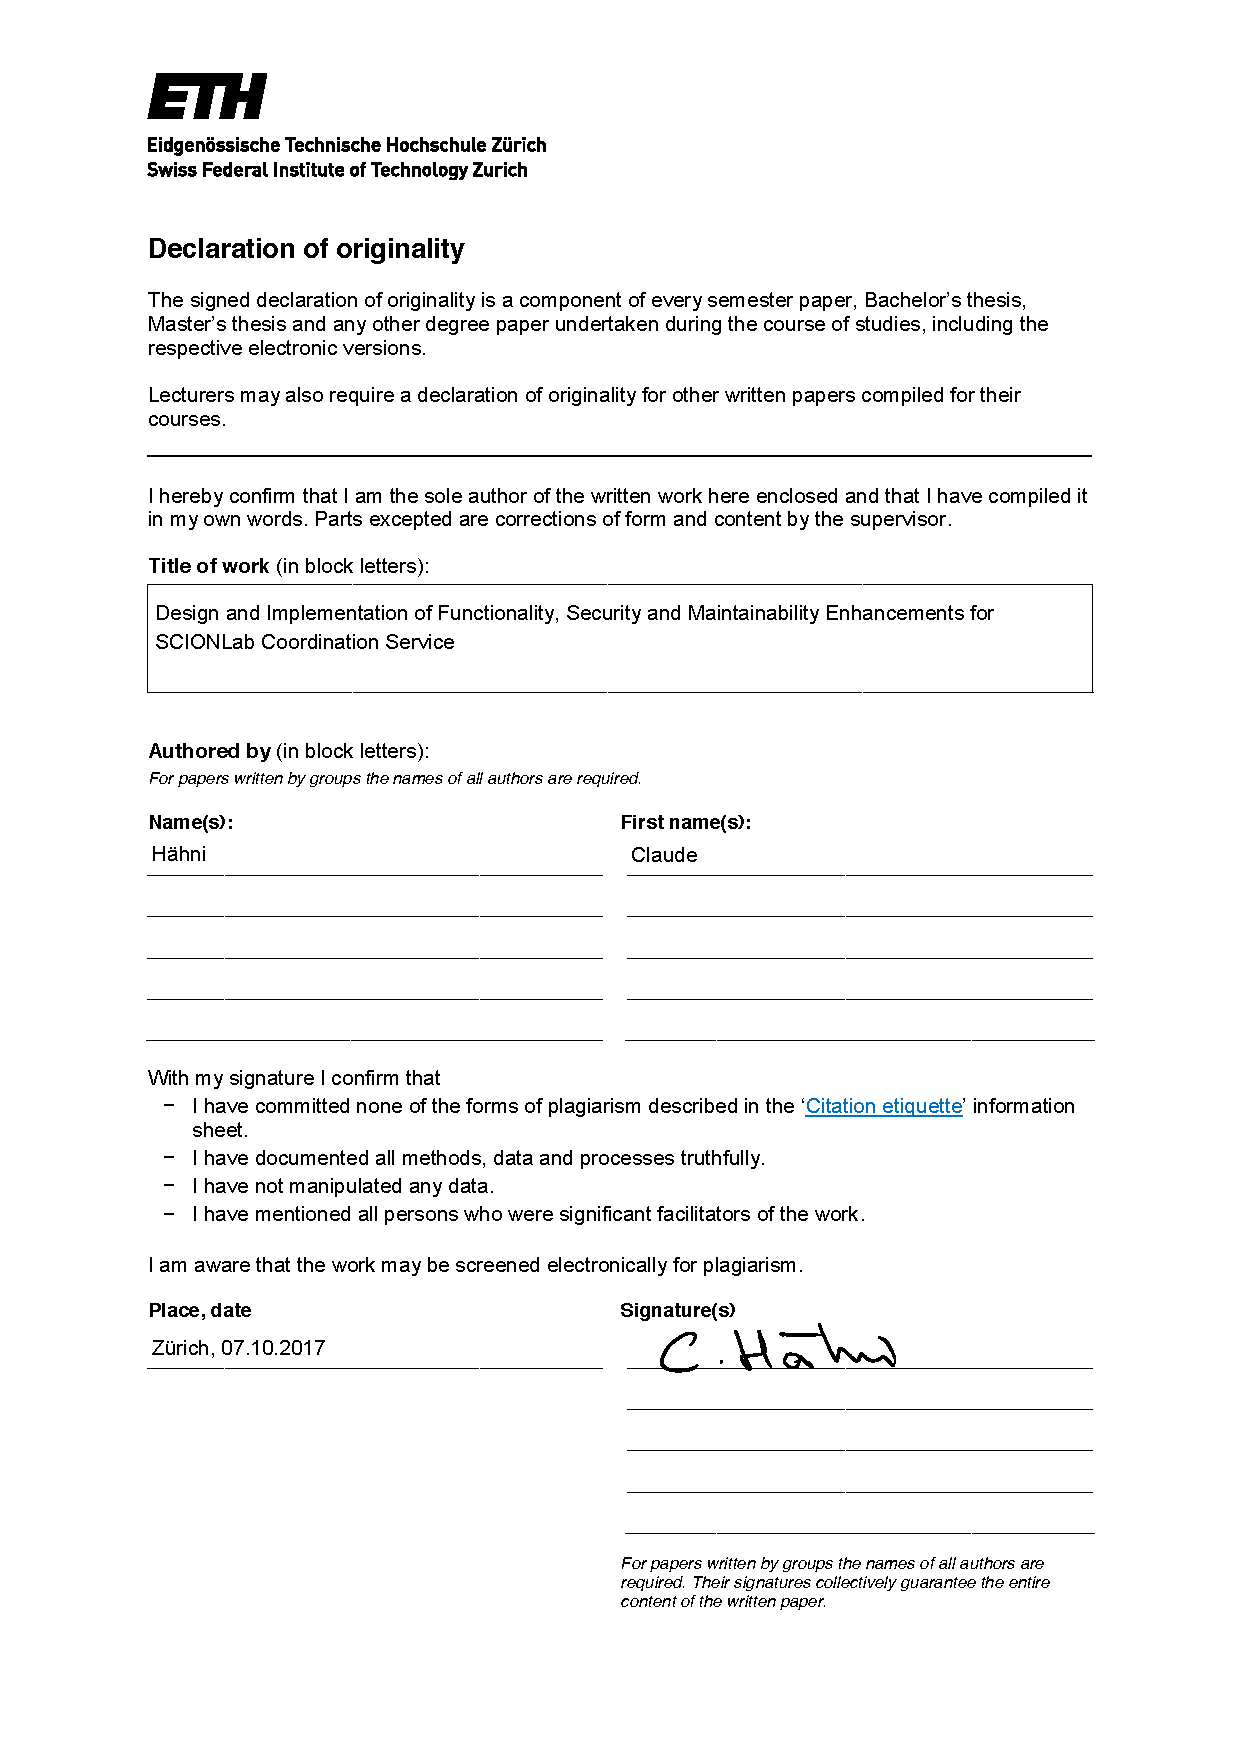
\includepdf[pages={-}]{declaration-originality.pdf}

\end{document}
